
\documentclass[../vs-script-first-v01.tex]{subfiles}
\graphicspath{{\subfix{../}}}
\begin{document}

\section{Einleitung}

Verteilte Systeme sind ein wichtiges Feld der Informatik, das sich mit der Vernetzung und Zusammenarbeit unabhängiger Computer beschäftigt, um in vielen Fällen eine gemeinsame Aufgabe zu erfüllen (kooperative Problemlösung). Durch die Verwendung von verteilten Systemen können komplexe Anwendungen und Aufgaben effektiver und effizienter gelöst werden, indem die Rechenleistung und Speicherkapazität mehrerer Computer gemeinsam genutzt werden. Dies muss aber nicht immer der Fall sein, wenn die Kosten den Nutzen übersteigen. Verteilte Systeme sind in vielen Bereichen der IT Branche, insbesondere im industriellen Umfeld, weit verbreitet und spielen eine wichtige Rolle bei der Entwicklung neuer Technologien und Anwendungen. Aktuell werden stark Themen wie Cloud Anwendungen, Künstliche Intelligenz, maschinelle Lernen oder auch des Internet of Things (IoT) diskutiert. Im Folgenden soll ein kleiner Einblick für Verteilte Systeme am Standort Hamburg gegeben werden, auf dem eine Definition des Begriffes \textbf{Verteilte Systeme}  mit einer angemessenen Abgrenzung folgt.

\subsection{Verteilte Systeme in Hamburg}

Die Stadt Hamburg ist ein wichtiger Wirtschaftsstandort in Deutschland und beherbergt zahlreiche Unternehmen, die auf innovative Technologien und Dienstleistungen angewiesen sind. In der Informatik haben sich verteilte Systeme als zentrales Konzept etabliert, um Innovationen	 mit komplexen Anwendungen und Dienste zu realisieren, insbesondere wenn diese über mehrere Standorte oder Rechenzentren verteilt sind.
\\\\
In Hamburg werden verteilte Systeme in verschiedenen Branchen eingesetzt, wie z.B. im Finanzsektor, im Gesundheitswesen, in der Logistik oder im öffentlichen Sektor. Dieser Text soll ein paar ausgewählte Beispiele aufzeigen.
\\\\
Der Hamburger Hafen ist einer der größten Häfen Europas und spielt eine wichtige Rolle im internationalen Handel. Mit dem Konzept des Smart Ports wird der Hafen als modernes und integriertes System betrachtet, das auf der Verwendung von verteilten Systemen und damit umgesetzte Prozesse basiert.
\examplevs{
Ein Smart Port ist ein System, das verschiedene Technologien und Konzepte integriert, um den Hafen effizienter, sicherer und nachhaltiger zu machen. Dazu gehören unter anderem Sensoren, Big-Data-Analysen, Cloud-Computing-Systeme und mobile Anwendungen. Alle diese Technogien können unter dem Aspekt Verteilte Systeme zusammengefasst werden.
}
Der Smart Port in Hamburg~\cite{HPA} wird von verschiedenen Partnern betrieben, wie z.B. der Hamburg Port Authority (HPA), Hafenunternehmen und IT-Dienstleistern. Die verteilten Systeme, die im Smart Port eingesetzt werden, ermöglichen es, Daten und Informationen in Echtzeit zu sammeln, zu analysieren und zu teilen. Dadurch können die Betriebsabläufe im Hafen optimiert und die Effizienz gesteigert werden.

\examplevs{
  Ein weiteres Beispiel für die Verwendung von verteilten Systemen im Smart Port ist das Hafenverwaltungssystem, das von der HPA betrieben wird. Das System besteht aus verschiedenen Modulen, die es ermöglichen, den Schiffsverkehr und die Lagerung von Waren im Hafen zu organisieren. Dazu gehören auch Funktionen zur Planung von Liegeplätzen und zur Überwachung von Sicherheitsaspekten.
  Technologien, die im Smart Port eingesetzt werden, sind u.a. Automatisierungstechnologien für Containerterminals und die Verwendung von Blockchain-Technologie zur Verbesserung der Sicherheit und Effizienz von Lieferketten. Alles dies sind wesentliche Technologien aus dem Kern der Verteilten Systeme.
}
Der Smart Port in Hamburg zeigt auf besondere Weise, wie verteilte Systeme mit weiteren innovative Technologien aus Maschinenbau oder Werkzeugbau  eingesetzt werden können\cite{Bockenfeld2020}, um komplexe Systeme wie einen Hafen zu optimieren und nachhaltiger zu gestalten.
\\\\
Auch die Luftfahrtindustrie, wie Airbus, setzt eine Vielzahl von verteilten Systemen ein, um Flugzeuge sicher und effizient zu betreiben. Ein verteiltes System in einem Flugzeug umfasst eine Vielzahl von Technologien, die es ermöglichen, verschiedene Komponenten und Systeme miteinander zu vernetzen, um eine reibungslose Kommunikation und Zusammenarbeit zu gewährleisten\cite{chen2017distributed}. Weitere Beispile sind z.B. Navigationssysteme, Autopiloten, Flugsicherheitssysteme oder auch Flugüberwachungssysteme. Diese Systeme kommunizieren miteinander über verschiedene Netzwerke, wie z.B. CAN-Bus/Realtime-Ethernet, Ethernet und WLAN und müssen zeitlich und örtlich koordiniert werden, wie auch den internationalen Anforderungen entsprechen.
\\\\
Die Verwendung von verteilten Systemen in der Luftfahrtindustrie hat zahlreiche Vorteile, wie z.B. die Verbesserung der Flugsicherheit, die Steigerung der Effizienz und die Reduzierung von Ausfallzeiten. Allerdings gibt es auch Herausforderungen, wie z.B. die Notwendigkeit einer sorgfältigen Planung und Integration sowie die Gewährleistung der Datensicherheit und des Datenschutzes. Ein Beispiel für ein verteiltes System in einem Flugzeug ist das Fly-by-Wire-System. 
\examplevs{
Das Fly-by-Wire-System ist ein elektronisches Steuerungssystem, das den mechanischen Steuermechanismus durch eine elektronische Steuerung ersetzt\cite{tian2017fault}. Das System besteht aus mehreren Komponenten, die miteinander kommunizieren und koordinieren, um das Flugzeug zu steuern. Die Komponenten sind über verschiedene Netzwerke, wie z.B. Ethernet\cite{wang2018architecture}, miteinander verbunden.
}
Weitere Technologien, die in diesem Kontext in Flugzeugen eingesetzt werden, sind u.a. Avionik-Systeme, die Daten zur Flugsicherheit sammeln und verarbeiten, oder auch Funksysteme.
\\\\
Ein weiteres, wichtiges Standbein für Hamburg ist der Kaufmanns-, Finanz- und Versicherungssektor. Hier spielen verteilte Systeme eine außergewöhnliche und immer stärkere Rolle. Ein Beispiel ist im Finanzwesen das Real-Time Gross Settlement System (RTGS)\cite{rtgs}, das von Zentralbanken auf der ganzen Welt eingesetzt wird. Dieses System ermöglicht die sofortige Übertragung von großen Geldbeträgen zwischen Banken und anderen Finanzinstitutionen in Echtzeit. RTGS nutzt eine verteilte Datenbank, um alle Transaktionen aufzuzeichnen und sicherzustellen, dass alle Parteien die gleichen Informationen haben.
\examplevs{
Auch das Clearinghaus-System\cite{clearinghouse}, das von Finanzinstitutionen und Versicherungen genutzt wird, um Transaktionen abzuwickeln und Zahlungen zu verarbeiten, ist erwähnenswert. Das System nutzt eine verteilte Datenbank, um alle relevanten Informationen zu speichern und zu verarbeiten, um sicherzustellen, dass alle Parteien korrekt abgerechnet werden.
}
Ein Zeitgeist Thema sind Blockchain\cite{blockchain} oder AI/KI-Systeme, welche in der Logistik-, Finanz- und Versicherungsbranche immer beliebter werden. Blockchain-Systeme nutzen eine verteilte Datenbank, um Transaktionen aufzuzeichnen und sicherzustellen, dass sie unveränderlich sind. Diese Technologie wird bereits in der Kryptowährungsbranche eingesetzt und findet auch in anderen Bereichen wie der Versicherung und der Verwaltung von Vermögenswerten Anwendung. AI-Systeme übernehmen immer mehr Themen in der Planung und Durchsetzung.
\\\\
Dies ist natürlich nur eine sehr kleine und nicht vollständige Auswahl von Beispielen und kann sicher um eine Vielzahl anderer Beispiele ergänzt werden. 


\newpage
\subsection{Definition}

Eine Definition~\cite{coulouris2012distributed} von verteilten Systemen ist beschrieben wie folgt: Man kann es als eine Gruppe von vernetzten, autonomen Computern verstehen, die gemeinsam eine Aufgabe erfüllen, ohne dass ein zentraler Koordinator benötigt wird. Dabei können die Computer geographisch verteilt sein und über unterschiedliche Hardware- und Software-Plattformen verfügen. Dies ist aber nur eine von vielen diskutierten, wobei sicher die folgende Definition die höchste Verbreitung hat: 

\warningvs{Laut Tanenbaum\cite{tanenbaum2017distributed} sind verteilte Systeme \enquote{eine Sammlung unabhängiger Computer, die den Benutzern als ein kohärentes System erscheinen} (Tanenbaum and van Steen, 2017, S. 4). Die Kommunikation in verteilten Systemen erfolgt über das Netzwerk und erfordert eine koordinierte Zusammenarbeit der einzelnen Komponenten.}
\mbox{}\\
Die Definition von einem Verteilten System ist somit nicht trennscharf. Es existieren, zu den genannten, durchaus alternative Definitionen, denen man sich im Zweifelsfall gewahr werden muss. So können beispielhaft für detailreichere Alternativen folgende genannt werden:

\examplevs{
So definiert \cite{garg2016distributed} ein verteiltes System als mehrere unabhängige Computer, die miteinander kommunizieren und \enquote{kooperieren}, um gemeinsam eine Aufgabe zu erfüllen.
\\
Anders sieht es \cite{mukherjee2015distributed}, wo der Fokus mehr auf die technologische Komponente gelegt wird. Hier ist ein verteiltes System \enquote{ein Netzwerk} aus autonomen Computern, die miteinander kommunizieren und koordiniert zusammenarbeiten, um eine gemeinsame Aufgabe zu erfüllen.
}
Sicher ist, es gibt viele verschiedene Definitionen von verteilten Systemen, die sich je nach Autor, Kontext und Zweck leicht oder stark unterscheiden können. Die grundlegende Idee hinter allen Definitionen ist jedoch die gleiche: 

\warningvs{Es geht um die Vernetzung und Zusammenarbeit unabhängiger Recheneinheiten, die keinen gemeinsamen Speicher nutzen.}

Nun kann man anführen, dass bei einer Vielzahl von Definitionen diese ihre Bedeutung verlieren, da ein effizienter und sinnvoller Einsatz in einer praktischen Umsetzung nicht hilfreich erscheint, doch ist hier folgendes anzuführen:

Verteilte Systeme bieten generische Lösungsansätze für \textbf{unterschiedliche Problemklassen} an. Da es sich bei Verteilten Systemen nicht selten um komplexe Systeme handelt, welche aus einer Vielzahl von miteinander kommunizierenden und kooperierenden Komponenten bestehen, haben die Abweichungen der Eigenschaften einen hohen Einfluss auf die Etablierung der generischen Lösungsansätze. Somit muss die doch meist sehr generische Definition um einzelne Eigenschaften angereichert werden, damit entsprechende Logikzweige für eine adäquate Lösung formuliert werden können. Die generische Definition ist daher als Ausgangspunkt zu sehen, für den weiteren Anforderungsprozess. 

Noch einen Schritt weiter, ist es besonders fordernd für den Anforderungsprozess, dass diese Eigenschaften der Komponenten auf verschiedenen Geräten und Standorten verteilt sein können und zunächst systematisch erfasst und vollständig beschrieben werden müssen. Fehler in diesem Prozess können weitreichende Folgen für den Erfolg der angestrebten Lösung haben.
\examplevs{
Um die Herausforderung zu verdeutlichen, soll die Aufgabe der Wegesuche in einem Labyrinth herangezogen werden. Die Aufgabe kann sehr einfach nachvollzogen werden, wenn man folgenden Algorithmus, auch bekannt als Breitensuche, etabliert.

\begin{itemize}
  \item Legen Sie eine Warteschlange an und fügen Sie den Startknoten hinzu.

  \item Solange die Warteschlange nicht leer ist, nehmen Sie den Knoten am Anfang der Warteschlange und prüfen Sie, ob es der Zielknoten ist. Wenn ja, haben Sie den Pfad zum Ziel gefunden und können den Algorithmus beenden.

  \item Andernfalls fügen sie alle unbesuchten Nachbarknoten des aktuellen Knotens zur Warteschlange hinzu und markieren sie als besucht.

  \item Wiederholen Sie Schritt 2 und 3, bis Sie den Zielknoten gefunden haben oder alle Knoten besucht wurden.
\end{itemize}
Diese Lösung ist trivial und durchläuft das Labyrinth schrittweise, indem der Algorithmus zuerst alle Knoten in der Nähe des Startknotens besucht, dann alle Knoten in der Nähe dieser Knoten, und so weiter, bis er den Zielknoten erreicht oder alle Knoten besucht wurden.
}
\examplevs{
Die Herausforderung in diesem Fall ist nicht das Verständnis für den Algorithmus, sondern die Herausforderung beginnt im Anforderungsprozess des verteilten Systems. Es ist wichtig zu beachten, dass der vorgestellte Lösungsansatz nur funktioniert, da das Labyrinth als Graph modelliert werden konnte, und der Informatiker dies in der Anforderungsanalyse erkennt. Wobei im verteilten System die Knoten als Positionen im Labyrinth und die Kanten, als  möglichen Wege, willkürlich verteilt sein können und somit die Herausforderung darin besteht, dass das ganze Bild des Labyrinths nicht direkt ersichtlich ist. So ist aber für eine adäquate Lösungsfindung genau diese Identifikation wesentlich, damit der mit der Lösung verbundene Graph und die damit verbundene Breitensuche als Logikbaum für eine effiziente Lösung identifiziert werden kann.
}

\examplevs{
Für ein verteiltes System mag bereits dies eine interessante Herausforderung für die Skalierung über die Problemgröße  darstellen und der parallelisierbarkeit des Problems, wahrscheinlicher ist jedoch, dass das Problem noch nicht vollständig erfasst ist. So ist es in einem verteilten System (VS)  nicht unerwartet das keine "Gottessicht" auf das Problem existiert und niemand den gesamten Graphen überblicken und organisieren kann.  In einem VS ist es ein wahrscheinliches Szenario, dass jeder Knoten gemeinsam mit anderen Knoten die Entscheidung über die Durchführung der Graphdurchsuchung organisieren muss, ohne sich seiner eigenen globalen Position bewusst zu sein. Dies erfordert eine sorgfältige Koordination und einen intensiven Informationsaustausch mit den benachbarten Knoten. Die Lösungsstrategie wird sich sicherlich unterscheiden, je nachdem, ob das System über stabile und verlustfreie Kommunikationswege verfügt oder ob der Graph instabil ist, beispielsweise weil er sich zur Laufzeit verändert oder Knoten unerwartet aus dem Verbund ausscheiden.
}
Die Bandbreite von Anwendungen und ihren Anforderungen, die verteilte Systeme nutzen, ist enorm und reicht - wie alleine für Hamburg festgestellt - von großen Online-Transaktionssystemen bis hin zu drahtlosen Sensornetzwerken. Es ist häufig sehr viel komplexer als die Suche nach einem Ausgang in einem Labyrinth oder die Identifikation einer einzelnen Problemklasse. Daher ist es wichtig, eine Definition und eine klare Abgrenzung zu schaffen, um sicherzustellen, dass die Systeme im Sinne einer notwendigen Verteilung effektiv entworfen, entwickelt und implementiert werden können. 

\warningvs{Hier werden jedoch oft Fehler gemacht, da nicht selten generische Ansätze ohne Berücksichtigung des Anwendungsfalls diskutiert werden und somit möglicherweise nicht zur angestrebten Lösung passen, da sie die notwendigen Charaktereigenschaften nicht repräsentieren. Somit ist die Erweiterung der Definition des vorhandenen verteilten Systems grundsätzlich eine Aufgabe die zu erfüllen ist, unabhängig des Startpunktes der gewählten generischen Definition.}
\examplevs{
Die Untersuchung der Eigenschaften von verteilten Systemen ist auch für die Forschung und Entwicklung noch immer sehr relevant.
}
Dennoch, am Anfang braucht man für den gesamten Prozess einen Startpunkt. Der Informatiker muss sich bewusst machen, dass die zu lösende Aufgabe ein verteiltes System repräsentiert. Für eine erste Einschätzung der Situation, ob das Themengebiet der verteilten Systeme zum Tragen kommt, genügt aber ein kleiner Schritt. Dieser Schritt umfasst die Prüfung einer wesentlichen Eigenschaft, die alle Definitionen miteinander verbindet.  Kurz gesprochen ist der gemeinsame Nenner das \enquote{nicht-vorhanden-sein} eines gemeinsamen (Arbeits-)Speichers. Wird kein gemeinsamer Speicher genutzt, um sich zu koordinieren, ist die Umsetzung eines verteilten Systems sehr wahrscheinlich und der Startpunkt gegeben, um die Anforderungen an das System und damit die genutzte Definition entsprechend zu verfeinern.
\warningvs{
Muss man kein VS bauen, sollte man es auch nicht tuen!
}
\subsection{Abgrenzung}
Eine Abgrenzung des Begriffs \enquote{Verteilte Systeme} in der Informatik kann nur auf unterschiedlichen Ebenen gelingen, da es sich bei Verteilten Systemen um ein sehr breites und vielschichtiges Feld handelt. Hier soll auch kein Versuch unternommen werden dies vollständig zu tun, sondern es soll nur einen Blick in diese Diskussion geben.
\\\\
Die Abgrenzung des Begriffs hängt davon ab, auf welcher Ebene man das verteilte System betrachtet und welche spezifischen Merkmale und Eigenschaften man berücksichtigen möchte. Eine klare Abgrenzung ist - wie bereits ausgeführt - wichtig, um sicherzustellen, dass die Systeme effektiv entworfen, entwickelt und implementiert werden können.

\subsubsection{Verteiltes und monolithisches System}

Auch wenn dieses Dokument sich primär auf die Umsetzung von verteilten Systemen konzentriert, darf nicht vergessen werden, dass dieser nur ein Kontext von vielen ist. Ein sehr bekanntes Architekturmodell welches man als Alternative zum Verteilten System verstehen kann, ist das monolithische System\cite{Newman2015}.
\\\\
Ein \textbf{monolithisches} System mit Fokus auf die Anwendung\cite{Szyperski2002} ist eine Softwarearchitektur, bei der alle Komponenten einer Anwendung in einer einzigen, großen Codebase zusammengefasst sind. Es gibt keine klare Trennung zwischen den einzelnen Komponenten, sondern alle Funktionen und Prozesse laufen innerhalb des gleichen Prozesses und können auf gemeinsame Ressourcen zugreifen. Im Gegensatz zu Verteilten Systemen gibt es keine Notwendigkeit, die Kommunikation zwischen verschiedenen Rechnern oder Prozessen zu koordinieren, da alles in einem einzigen Prozess läuft. Monolithische Systeme waren lange Zeit die Standardarchitektur für Softwareanwendungen, bevor Verteilte Systeme aufkamen.
\\\\
Ein monolithisches System ist in der Regel einfacher zu entwickeln, zu testen und zu deployen als ein Verteiltes System. Es ist auch einfacher, die Performance und Skalierbarkeit des Systems zu optimieren, da alles in einer einzigen Anwendung läuft. Außerdem gibt es weniger komplexe Interaktionen und weniger Schnittstellen zwischen den Komponenten, was die Wartung und das Debugging erleichtert. Dies sind klare Argumente für die Wahl der Architektur in der Praxis, wenn eine Wahl besteht.
\\\\
Ein weiterer Vorteil eines monolithischen Systems ist, dass es in der Regel eine bessere Sicherheit und Zuverlässigkeit bietet, da es einfacher ist, das System als Ganzes zu überwachen und zu sichern. Bei Verteilten Systemen kann es schwieriger sein, alle Komponenten zu überwachen und zu sichern, da sie möglicherweise über verschiedene Netzwerke und Standorte verteilt sind.
\\\\
Allerdings hat ein monolithisches System auch einige Nachteile. Es kann schwieriger sein, neue Technologien und Tools zu integrieren, da das gesamte System angepasst werden muss. Außerdem kann es schwieriger sein, das System auf verschiedene Umgebungen zu skalieren und zu verteilen, da es als Ganzes betrachtet wird.
\\\\
Als ein klassischer extremer \textbf{Gegenentwurf} aus Sicht der Softwarearchitektur \textbf{zum monolithischen} System kann aus dem Kontext der Verteilten Systeme auch die Microservice-Architektur\cite{fowler2014microservices} betrachtet werden.
\examplevs{{}
Eine Microservice-Architektur ist eine spezielle Form der Verteilten Systeme, bei der eine Anwendung in einzelne unabhängige Komponenten (Services) aufgeteilt wird. Jeder Service ist in der Regel für eine bestimmte Funktion verantwortlich und kann separat entwickelt, getestet, bereitgestellt und skaliert werden. Die Services kommunizieren über definierte Schnittstellen miteinander und werden oft in Containern bereitgestellt.
\\\\
Somit kann man sagen, dass eine Microservice-Architektur ein Verteiltes System darstellt, da die Services auf verschiedenen Servern oder in verschiedenen Containern laufen und über das Netzwerk miteinander kommunizieren. Die Vorteile eines Verteilten Systems, wie Skalierbarkeit, Ausfallsicherheit und Flexibilität, gelten auch für eine Microservice-Architektur. Allerdings bringt die Komplexität der Kommunikation zwischen den Services auch zusätzliche Herausforderungen mit sich, wie z.B. die Sicherstellung der Konsistenz und Verfügbarkeit der Daten. Diese Herausforderungen hat ein monolithisches System nicht.
}

\subsubsection{Verwandte Großrechner/Mainframes}
Ein Großrechner ist ein leistungsstarkes Computersystem, das typischerweise in einem Rechenzentrum betrieben wird und für die Verarbeitung von großen Datenmengen und rechenintensiven Aufgaben wie Simulationen, wissenschaftlichen Berechnungen oder Geschäftsanwendungen verwendet wird. Ein Großrechner zeichnet sich durch seine hohe Leistung, Zuverlässigkeit, Verfügbarkeit und Sicherheit aus. Großrechner werden oft in großen Unternehmen, Regierungsbehörden oder Forschungseinrichtungen eingesetzt.
\\\\
Im Gegensatz zu Großrechnern sind verteilte Systeme ein Netzwerk von miteinander verbundenen Computern, die koordiniert arbeiten, um eine gemeinsame Aufgabe zu erfüllen. Verteilte Systeme sind darauf ausgelegt, Last und Ressourcen auf mehrere Computer zu verteilen und können von kleinen Netzwerken bis hin zu globalen Netzwerken von Millionen von Computern reichen. Verteilte Systeme können für verschiedene Anwendungen eingesetzt werden, darunter verteilte Datenbanken, verteilte Rechen- und Speicherressourcen, Webanwendungen und Cloud Computing.
\\\\
Der Hauptunterschied zwischen einem Großrechner und einem verteilten System liegt in der Art und Weise, wie die Ressourcen bereitgestellt werden. Ein Großrechner verfügt über eine leistungsstarke Architektur und eine hohe Anzahl von Speicher- und Ein-/Ausgabe-Subsystemen, die mit Hochgeschwindigkeitsverbindungen verbunden sind. Ein verteiltes System hingegen besteht aus vielen Computern, die miteinander verbunden sind und zusammenarbeiten, um eine Aufgabe zu erfüllen.
\\\\
Ein weiterer Unterschied besteht in der Art und Weise, wie die Ressourcen verwaltet werden. Ein Großrechner verfügt normalerweise über einen dedizierten Systemadministrator, der für die Verwaltung der Hardware und Software des Systems verantwortlich ist. Verteilte Systeme hingegen sind oft dezentralisiert und verfügen über eine gemeinsame Management-Infrastruktur, die die Ressourcen überwacht und verwaltet.

\subsubsection{Abstraktionsebenen}
Eine klare Definition von Verteilten Systemen fällt insbesondere auch daher schwer, da Verteilte Systeme nicht immer eine vergleichbare abstrahierte Struktur aufweisen. Stattdessen können verschiedene Abstraktionsansätze auf unterschiedlichen Ebenen für die Analyse eines Verteilten Systems angenommen werden. 

Um diese unterschiedlichen Ebenen zu verdeutlichen, soll zunächst die Unterscheidung in zwei Ebenen angedacht werden, auch wenn eine Vielzahl anderer Einteilungen angenommen werden können.
\\\\
So können verteilte Systeme in einem ersten trivialen Ansatz von einer technologischen und einer anwendungsbezogenen Ebene betrachtet werden \cite{coulouris2012distributed}. Auf der technologischen Ebene werden Verteilte Systeme als eine Sammlung von Computern und Netzwerken interpretiert, die miteinander kommunizieren und kooperieren, um eine gemeinsame Aufgabe zu erfüllen. Diese Art der Interpretation wurde bereits bei den Begriffsbestimmungen diskutiert. Auf der anwendungsbezogenen Ebene geht es dagegen um die Verwendung von Verteilten Systemen zur Lösung von Problemen in bestimmten Anwendungsdomänen.

\examplevs{Ein Beispiel für ein verteiltes System auf technologischer Ebene ist das Internet. Das Internet besteht aus einer Vielzahl von Computern und Netzwerken, die miteinander verbunden sind und Informationen austauschen.
 Andere Beispiele für verteilte Systeme auf technologischer Ebene sind Cloud-Computing-Plattformen, Peer-to-Peer-Netzwerke und verteilte Datenbanken.
}
Auf der anwendungsbezogenen Ebene gibt es ebenfalls eine Vielzahl von Anwendungen, die auf Verteilten Systemen basieren, wie Facebook oder X. 
\examplevs{
Ein Beispiel hierfür sind Social-Media-Plattformen wie Facebook und X, die auf einer verteilten Architektur aufgebaut sind und es Benutzern ermöglichen, Informationen und Nachrichten auszutauschen. Andere Beispiele für Verteilte Systeme auf anwendungsbezogener Ebene sind E-Commerce-Plattformen oder Anwendungen im Gesundheitswesen.
}
Da dieses Dokument primär in der Lehre eingesetzt werden soll, wird der Begriff für die Angewandte Informatik (AI) und der Informatik für Technische Systeme (ITS) diskutiert.

\subsubsection{Verteilte Systeme in AI und ITS}

Die Unterscheidung zwischen Verteilten Systemen in der eher technischen Informatik und in der angewandten Informatik ist nicht immer klar abzugrenzen, da beide Bereiche sich oft überschneiden. Es gibt jedoch einige Unterschiede, die man beachten kann.
\\\\
In der technischen Informatik geht es hauptsächlich um die Entwicklung von Technologien und Infrastrukturen, wie z.B. Netzwerkprotokollen und verteilten Datenbanken \cite{coulouris2012distributed}. Der Schwerpunkt liegt hier auf der Entwicklung von effizienten und zuverlässigen Algorithmen und Protokollen für verteilte Systeme. Auf der anderen Seite konzentriert sich die angewandte Informatik auf die Anwendung von verteilten Systemen in verschiedenen Anwendungsbereichen wie E-Commerce, E-Government, und Cloud Computing \cite{ghosh2012distributed}. Der Schwerpunkt liegt hier auf der Anwendung von vorhandenen Technologien und Infrastrukturen für Verteilte Systeme, um konkrete Probleme zu lösen.
\\\\
Ein weiterer nicht unerheblicher Unterschied besteht darin, dass Verteilte Systeme in der technischen Informatik oft auf die Forschung und Entwicklung von neuen Technologien und Algorithmen fokussiert sind, die in den Schnittstellen eine hohe Nähe zu Hardwareentwicklern aufweisen, während Verteilte Systeme in der angewandten Informatik oft eine größere Rolle bei der Umsetzung von Geschäftsprozessen spielen und somit nicht selten eng mit dem Management von Unternehmen verbunden sind\cite{birman2012guide}.

\subsubsection{Aspekte und Sichten}
Bisher lag der implizierte Fokus der Diskussion primär auf den Aspekten des Designs und der Architektur von Verteilten Systemen sowie der technologischen Basis, wie sie in Netzwerkprotokollen und -kommunikation zu finden ist. Darüber hinaus können jedoch auch andere Aspekte genannt werden, unter denen ein Verteiltes System diskutiert werden kann \cite{tanenbaum2017distributed}.
\begin{itemize}
  \item \textbf{Skalierbarkeit und Ausfallsicherheit}: Verteilte Systeme sollen nicht selten in der Lage sein -  mit steigender Last, bei Ausfällen oder Fehlern - selbst in Teilen weiterhin zu funktionieren. Hierzu müssen spezifische Skalierungs- und Wiederherstellungsmechanismen implementiert werden.
  \item \textbf{Datenmanagement:} In Verteilten Systemen müssen Daten effektiv verwaltet und zwischen verschiedenen Komponenten ausgetauscht werden. Hierbei müssen spezifische Datenmanagement- und -konsistenzmechanismen implementiert sein, die einen neuen Umgang mit Konsistenz erfordern.
  \item \textbf{Orchestrierung und Deployment:} In Verteilten Systemen müssen die verschiedenen Komponenten orchestriert und deployed werden, um eine reibungslose Kommunikation und Zusammenarbeit zu gewährleisten. Hierbei müssen spezifische Orchestrierungs- und Deployment-Mechanismen definiert und implementiert werden. Auch das Testen bringt hier neue Herausforderungen.
  \item \textbf{Sicherheit:} In Verteilten Systemen müssen Maßnahmen ergriffen werden, um die Sicherheit der übertragenen Daten und der beteiligten Systeme zu gewährleisten. Dazu gehören Authentifizierung, Verschlüsselung und Schutz vor Angriffen. Dies ist eine sehr wichtige Sicht auf das System, auch wenn es kein zentraler Fokus dieser Ausarbeitung ist.
\end{itemize}
Alle Aspekte implizieren unterschiedliche Anforderungen, die disjunkt betrachtet werden können, aber nicht selten in einer Interaktion und Abwägung zueinanderstehen, was eine weitere Komplexität für diesen bereits intensiven Entwicklungsprozess einbringt. Auch Aspekte aus der Organisation eines Entwicklungsteams selbst geben immer wieder neue Impulse, um die Herausforderungen von Verteilten Systemen neu zu interpretieren und zu diskutieren. Diese Diskussionen geben gerne eine Einteilung in Rollen und Sichten vor. Ein Versuch ein Verteiltes System in Sichten einzuordnen, soll in der folgenden Aufzählung versucht werden:
\importantvs{
  \begin{itemize}
    \item \textbf{Architektursicht:} Hier liegt der Fokus auf der Struktur und Organisation des Systems sowie der Verteilung der Komponenten und deren Interaktion. Es geht darum, die Komponenten des Systems zu identifizieren, deren Aufgaben und Verantwortlichkeiten zu definieren und eine geeignete Architektur zu entwerfen, die eine effiziente Zusammenarbeit der Komponenten ermöglicht.
  \end{itemize}
}    
\importantvs{
  \begin{itemize}    
    \item \textbf{Prozesssicht:} In der Prozesssicht steht die zeitliche Abfolge der Abläufe und Interaktionen im Vordergrund. Es geht darum, die Prozesse und Workflows im System zu identifizieren und zu modellieren, um eine effektive Koordination und Steuerung der Aktivitäten zu gewährleisten.
  \end{itemize}
}    
\importantvs{
  \begin{itemize}    
    \item \textbf{Datensicht:} Die Datensicht fokussiert auf die Daten, die im System verarbeitet werden. Hier geht es um die Definition und Modellierung der Datenstrukturen, die in den Komponenten des verteilten Systems verwendet werden, sowie um die Speicherung, Verarbeitung und Übertragung der Daten.
  \end{itemize}
}    
\importantvs{
  \begin{itemize}     
    \item \textbf{Sicherheitssicht:} Die Sicherheitssicht betrachtet die Aspekte der Datensicherheit und des Datenschutzes im Verteilten System. Es geht darum, Risiken und Bedrohungen zu identifizieren und geeignete Maßnahmen zu ergreifen, um die Daten und das System insgesamt vor unautorisiertem Zugriff, Missbrauch oder Diebstahl zu schützen.
  \end{itemize}
}    
\importantvs{
  \begin{itemize}     
    \item \textbf{Betriebssicht:} Die Betriebssicht betrachtet Aspekte wie die Verfügbarkeit, Zuverlässigkeit und Skalierbarkeit des Verteilten Systems. Hier geht es darum, sicherzustellen, dass das System kontinuierlich und zuverlässig arbeitet und bei Bedarf flexibel skaliert werden kann.
  \end{itemize}
}    
\importantvs{
  \begin{itemize}     
    \item \textbf{Entwicklersicht:} Die Entwicklersicht betrachtet Aspekte der Entwicklung und Implementierung von Verteilten Systemen. Hier geht es um die Auswahl geeigneter Programmiersprachen, Frameworks und Tools sowie um die Anwendung von Best Practices und Methoden, um eine effiziente und qualitativ hochwertige Entwicklung zu gewährleisten.
  \end{itemize}
}
Je nach Kontext und Zielsetzung können auch weitere Sichten auf ein Verteiltes System relevant sein, beispielsweise die ökonomische bzw. ökologische Sicht oder die Benutzersicht. Auch hier können die einzelnen Diskussionspunkte eine beliebige Komplexität annehmen. Wichtig ist, im Vorfeld einer Diskussion zu bestimmen welcher Fokus die Diskussion hat. Alles miteinander zu verweben, ist eine sehr komplexe Herangehensweise, die nicht selten zum Scheitern verurteilt ist.
\warningvs{
Das Teile-und-herrsche Verfahren ist hier ein erster guter Ansatz, um Arbeitspakete und Aufgabenfelder zu schnüren.
}
Als Beispiel soll die ökonomische/ökologische Anforderung an den Energieverbrauch von Transaktionen eingebracht werden. Es ist schwierig vorab eine generische, aber genaue Antwort auf diese Frage zu geben, da dies von vielen Faktoren abhängig ist, wie z.B. der Art der Datenbank, der Größe und Komplexität der Transaktionen und der Energiequelle, die zur Unterstützung der Datenbank verwendet wird.
Soll weiter die Anforderung an die \ce{CO2} Produktion ausgerichtet werden, gibt es schon vieles alleine bei der Datenhaltung zu beachten. 
\examplevs{
Beispielhaft gibt es einige Schätzungen und Studien, die einen Vergleich zwischen der Energieeffizienz von Datenbanktransaktionen und Blockchain-Transaktionen ermöglicht. Laut einer Studie von PwC Deutschland aus dem Jahr 2019\cite{pwc2019} benötigt eine durchschnittliche Bitcoin-Transaktion etwa 550 kWh, um verarbeitet zu werden. Zum Vergleich: Eine einzelne Visa-Transaktion benötigt nur 0,002 kWh. Dies bedeutet, dass Sie mit einer einzigen Blockchain-Transaktion Hunderte oder sogar Tausende von Datenbanktransaktionen durchführen könnten, um die gleiche Menge an Energie zu verbrauchen.
}
\examplevs{
Es ist jedoch auch wichtig zu beachten, dass die Energieeffizienz von Blockchain-Transaktionen zunehmend verbessert wird, insbesondere durch den Einsatz von Proof-of-Stake-Konsensmechanismen anstelle des energieintensiven Proof-of-Work. Die Verfahren werden in dieser Ausarbeitung noch miteinander besprochen und diskutiert. Darüber hinaus können Datenbanken selbst auch energieeffizienter gestaltet werden, indem Anfragen umgebaut oder generell die Energiequelle auf erneuerbare Energiequellen geändert wird. Auch ein Umstieg auf energieeffiziente Hardware ist denkbar.
}
Aber selbst wenn man beispielhaft mit dem Teile-und-herrsche Ansatz erfolgreich die Teilaspekte beleuchtet, darf man dabei das gesamte System nicht aus dem Auge verlieren. Sichten wirken aufeinander. Dies ist auch stark erkennbar in moderneren Entwicklungsmethoden, wo versucht wird verschiedene Sichten natürlich im (Entwicklungs-)Prozess zu vereinen. Als Anwendungsbeispiel aus der Praxis kann die Entwicklersicht mit der Betriebssicht verbunden werden. DevOps\cite{kumar2016devops} ist eine Variante die in diesem Kontext diskutiert werden kann.
\importantvs{DevOps ist eine agile Methode, die darauf abzielt, die Zusammenarbeit zwischen der Entwicklung (Dev) und dem Betrieb (Ops) von Software zu verbessern, um schnellere und zuverlässigere Softwarebereitstellungen zu erreichen.}

Verteilte Systeme führen sehr häufig zu komplexeren Architekturen, die eine engere Zusammenarbeit zwischen den Entwicklern und Betriebsteams erfordern. In einem Verteilten System müssen Entwickler und Betriebsteams sich auf die gemeinsame Verantwortung für die Verfügbarkeit, Leistung und Sicherheit der Systeme konzentrieren. Dies erfordert eine enge Zusammenarbeit und Kommunikation zwischen den Teilhabenden, um sicherzustellen, dass alle Aspekte des Systems effektiv und effizient verwaltet werden. Aus der Methode lassen sich dann weitere Praktiken, Werkzeuge und Technologien ableiten.
\examplevs{
DevOps-Praktiken, wie Continuous Integration (CI) und Continuous Delivery (CD) sind heute wichtige Schlagwörter, wobei die technologischen Lösungen in den Kontexten nicht selten wieder ein Verteiltes System darstellen. Durch die Automatisierung von Entwicklungs- und Bereitstellungsprozessen können Entwickler und Betriebsteams schnell auf Änderungen im System reagieren und sicherstellen, dass neue Funktionen und Updates ohne Unterbrechung der Systemleistung bereitgestellt werden können. Dies ist insbesondere wichtig bei Verteilten Systemen, da die Komplexität der Systeme die manuelle Verwaltung erschwert und Zeit und Ressourcen erfordert. Dieser Ansatz kommt aber auch mit Nachteilen, wie zum Beispiel hohe Einarbeitungskosten, kulturelle Herausforderungen (Dev und Ops) oder auch die neue Komplexität bei der Verbindung der Sichten.
}

\importantvs{Was am Ende aber bleibt ist, das die Entwicklung und Bereitstellung von Verteilten Systemen eine enge Zusammenarbeit aller Stakeholder mit ihren Sichten, sowie die Nutzung von  modernen Entwicklungspraktiken und Automatisierungstools, um sicherzustellen, dass die Systeme effektiv und effizient verwaltet werden.}
\newpage

\subsection{Ziele der Verteilten Systeme}
Für die weitere Diskussion soll zunächst angenommen werden, dass ein verteiltes System aus verschiedenen Komponenten besteht, aber mindestens zwei, die nicht über einen gemeinsamen Speicher verfügen. Weiter soll angenommen werden, dass für die Entwicklung verteilter Systeme zunächst die gleichen generischen Ziele gelten wie für ein nicht-verteiltes System. 
\examplevs{
Typische Ziele (Bekannt vielelicht aus SE), die in diesem Kontext gerne genannt werden, sollen im Folgenden nochmal aufgeführt werden.
\begin{itemize}
  \item \textbf{Funktionalität:} Die Software sollte die vom Benutzer erwarteten Funktionen bereitstellen und eine positive Benutzererfahrung bieten.
  \item \textbf{Zuverlässigkeit:} Die Software sollte zuverlässig sein und in verschiedenen Umgebungen stabil laufen, ohne Fehler zu verursachen oder unerwartet zu crashen.
  \item \textbf{Skalierbarkeit:} Die Software sollte in der Lage sein, sich an veränderte Anforderungen und eine wachsende Benutzerzahl anzupassen, ohne dass es zu Engpässen kommt.
  \item \textbf{Leistung:} Die Software sollte schnell und effizient arbeiten und eine gute Leistung bieten, auch bei großen Datenmengen.
  \item \textbf{Sicherheit:} Die Software sollte sicher sein und vertrauliche Daten schützen, indem sie Verschlüsselung, Zugriffskontrolle und andere Sicherheitsmaßnahmen implementiert.
  \item \textbf{Wartbarkeit:} Die Software sollte einfach zu warten und zu aktualisieren sein, indem sie gut strukturiert und kommentiert ist und eine gute Dokumentation bereitstellt.
  \item \textbf{Portabilität:} Die Software sollte auf verschiedenen Plattformen und Betriebssystemen laufen und kompatibel mit anderen Systemen und APIs sein.
  \item \textbf{Benutzerfreundlichkeit:} Die Software sollte einfach zu bedienen und zu verstehen sein und eine gute Benutzererfahrung bieten.
  \item \textbf{Anpassbarkeit:} Die Software sollte anpassbar sein und es Benutzern und Entwicklern ermöglichen, Funktionen hinzuzufügen oder zu ändern, um ihre Anforderungen zu erfüllen.
  \item \textbf{Kompatibilität:} Die Software sollte mit anderen Systemen und Anwendungen kompatibel sein, um die Integration und den Datenaustausch zu erleichtern.
\end{itemize}
%Die genannten Ziele in der Softwareentwicklung sind wichtig, weil sie dazu beitragen, sicherzustellen, dass die Software eine hohe Qualität und eine positive Benutzererfahrung bietet. Die Kriterien können auch entsprechend den Anforderungen an die Software erweitert oder auch unterschiedlich gewichtet werden. 
}
Eine Software, die nicht die erwartete Funktionalität bereitstellt oder unzuverlässig ist, kann dazu führen, dass Benutzer frustriert sind und das Vertrauen in die Software verlieren, dies gilt natürlich für verteilte Systeme im gleichen Maße. Eine Software, die langsam oder ineffizient arbeitet, kann die Produktivität der Benutzer beeinträchtigen und zu einem Verlust an Zeit und Geld führen.
\\\\
Wartbarkeit und Anpassbarkeit sind ebenfalls wichtige Ziele, da Software oft aktualisiert oder erweitert werden muss, um mit den sich ändernden Anforderungen und Technologien Schritt zu halten. Eine schlecht strukturierte oder dokumentierte Software kann die Wartung und Erweiterung erschweren und die Kosten für das Unternehmen erhöhen. Für den Aufbau eines Verteilten Systems ist dies essenziell, insbesondere die Anpassbarkeit da verschiedene unterschiedliche Systeme mitunter kooperativ zur Problemlösung beitragen müssen.
\\\\
Benutzerfreundlichkeit und Anpassbarkeit tragen ebenfalls zur Zufriedenheit der Benutzer bei und können die Akzeptanz und Nutzung der Software erhöhen. Dass dies auch für ein verteiltes System notwendig ist, kann nicht bestritten werden.
\\\\
Diese Ziele sollten im Prozess der Anforderungsanalyse auch das Gespräch mit den Stakeholdern bestimmen. 
\examplevs{
Ein Stakeholder im Entwicklungsprozess ist eine Person oder Gruppe, die von der Entwicklung und dem Einsatz der Software betroffen ist oder davon beeinflusst wird.
Es ist zu diesem Zeitpunkt wichtig verstanden zu haben, dass Stakeholder unterschiedliche Interessen und Anforderungen an das System haben und auch die Ziele unterschiedlich gewichten und beschreiben.
}
Die Herausforderungen im SE-Prozess sind bereits unabhägig einer Verteilung vielfältig und sollen im Folgenden nochmals am Beispiel der Ausfallsicherheit veranschaulicht werden. Ausfallsicherheit ist interessant, da sie als eigenständiges Ziel bereits für eine monolithische Lösung funktioniert, aber im Kontext eines verteilten Systems zusätzliche Dimensionen erhält:

\paragraph{Diskussion Ausfallsicherheit in SE}\mbox{}\\
Unbestritten ist, Ausfallsicherheit ist ein wichtiges Ziel. Typischerweise werden Anforderungen an Ausfallsicherheit in der Anforderungsbeschreibung der Anwendung, der Geschäfts- und/oder Service-Level-Vereinbarungen (SLAs) festgehalten. Zu bemerken ist hier bereits, dass in einem Verteilten System unterschiedliche Stakeholder mit unterschiedlichen Komponenten mit unterschiedlichen Vereinbarungen bestehen können. Die folgende Aufzählung soll nur einen beispielhaften Eindruck vermitteln:
\importantvs{
  \begin{itemize}
    \item Mission-critical Anwendungen: Für Anwendungen, die entscheidend für das Überleben von Organisationen oder Systemen sind, wird eine hohe Ausfallsicherheit gefordert. Hier sind hohe Verfügbarkeit, Redundanz, Lastverteilung, Fehlererkennung und -behebung von größter Bedeutung. Ein Ausfall kann zu hohen Verlusten oder sogar zu gefährlichen Situationen führen.

    \item Hochverfügbare Anwendungen: Hochverfügbare Anwendungen benötigen zwar keine 100\% ige Verfügbarkeit, jedoch müssen sie in der Lage sein, in kürzester Zeit wieder online zu gehen. Hier ist eine schnelle Fehlererkennung und -behebung sowie die Verwendung von Lastverteilung und Redundanztechniken entscheidend.

    \item Business-kritische Anwendungen: Für Anwendungen, die wichtige Geschäftsprozesse unterstützen, ist eine hohe Verfügbarkeit und Ausfallsicherheit erforderlich. Hier sind redundante Systeme, Backups, Failover-Systeme und ein schnelles Wiederherstellungsverfahren wichtig, um eine schnelle Wiederherstellung von Daten und Anwendungen nach einem Ausfall zu gewährleisten.

    \item Nicht-kritische Anwendungen: Für Anwendungen, die nicht kritisch sind, können die Anforderungen an die Ausfallsicherheit geringer sein. Hier können manuelle Backups, geringere Redundanz und längere Wiederherstellungszeiten akzeptabel sein.
  \end{itemize}
}
Je kritischer die Anwendung, desto höher sind die Anforderungen an die Ausfallsicherheit und desto stärker müssen Redundanz- und Wiederherstellungsstrategien auch in einem verteilten System implementiert werden. Dennoch ist noch nichts im eigentlichen Sinne über den Grad der Ausfallsicherheit gesagt. 
\warningvs{Erst wenn quantifizierbare, überprüfbare Kriterien formuliert werden, die Hülsenworte wie \enquote{hoch}, \enquote{schnell} und \enquote{wichtig} ersetzen, bekommen die Vereinbarungen einen Wert.}
Während bei einer Komponente eine schnelle Wiederherstellung mit 200 Millisekunden verbunden ist, kann bei einer anderen Komponente oder Technologie eine schnelle Wiederherstellung mit zwei Tagen verbunden sein. Auch \enquote{wichtig} kann eine kritische Formulierung sein, wenn es nicht genug Ressourcen, wie zum Beispiel dem Personal, gibt um alle Systeme mit der gleichen Priorisierung - \enquote{wichtig} - zu bearbeiten. Schwierige und harte Diskussionen können diese Detailfragen in sich tragen. In der Entwicklung der Verteilten Systeme muss man sich über die unterschiedlichen Dimensionen bewusst sein und die Stakeholder durch den Prozess begleiten.

Diese Diskussion kann noch weitergetrieben und mit Methoden und Werkzeugen bereichert werden, soll aber im ersten Schritt ausreichen, um die Anforderungen an den Prozess der Anforderungsanalyse zu verdeutlichen. 
\warningvs{Weiterhin ist nochmals darauf hingewiesen, dass die gleiche oder eine sehr ähnliche Diskussion auch für jedes weitere Ziel beschrieben werden kann.}

Besonders herausgehoben werden, soll auch nochmlas Sicherheit. Sicherheit ist in Verteilten Systemen ebenfalls von sehr großer Bedeutung, da vertrauliche Daten und Informationen durch fehlerhafte oder unsichere Software gefährdet werden können. Es ist wichtig, sicherzustellen, dass die Software alle erforderlichen Sicherheitsmaßnahmen implementiert, um den Schutz der Daten zu gewährleisten, dass dies eine besondere Herausforderung in einem verteilten System darstellen kann, wurde bereits ausgeführt und sollte in seiner Anforderung nicht unterschätzt werden. Auch wenn die Bedeutung nicht stark genug motiviert werden kann, ist es nicht Teil dieser Ausarbeitung und wird weiterführenden Modulen überlassen.
\\\\
Zu diesem Zeitpunkt möchten wir uns in diesem Dokument auf die Ziele konzentrieren, die nochmals eine besondere Bedeutung im Kontext der verteilten Systeme erhalten. Etabliert in diesem Kontext haben sich die Ziele von~\cite{tanenbaum2017distributed}:\footnote{Die Ziele werden im Detail im Folgenden nochmals genauer diskutiert werden.}
\warningvs{
\textbf{Ziele der Vertielten Systeme}
  \begin{itemize}
    \item Resource-Sharing
    \item Openness
    \item Scalability
    \item Distribution transparency
  \end{itemize}
}

\label{Woche01}

%\begin{itemize}
%\item Ressourcen-Sharing: Die Möglichkeit, Ressourcen wie Hardware, Software und Daten über ein Netzwerk hinweg gemeinsam zu nutzen, ist ein wichtiges Ziel für verteilte Systeme. Dies kann dazu beitragen, die Kosten für den Erwerb und Betrieb von Ressourcen zu senken und die Effizienz von Organisationen zu steigern.
%\item Offenheit: Verteilte Systeme sollen offen für verschiedene Arten von Hardware, Software und Netzwerkarchitekturen sein. Durch die Verwendung offener Standards und Protokolle können Systeme von verschiedenen Anbietern miteinander kommunizieren und interoperabel sein.
%\item Skalierbarkeit: Verteilte Systeme sollen in der Lage sein, sich an eine wachsende Anzahl von Benutzern und Ressourcen anzupassen und dabei eine gute Leistung zu bieten. Hierfür sind Skalierungstechniken wie Lastverteilung und Replikation notwendig.
%\item Transparenz: Dieses Ziel bezieht sich hier auf die Fähigkeit, dem Benutzer die Komplexität des Systems zu verbergen und ihm das Gefühl zu geben, als ob er auf ein einziges, zusammenhängendes System zugreift.
%\end{itemize}	


\subsubsection{Ressourcen-Sharing}
Das Ziel des Ressource-Sharings in verteilten Systemen bezieht sich darauf, dass Ressourcen wie Hardware, Software und Daten zwischen verschiedenen Knoten und Anwendungen im System geteilt werden können. Durch das Teilen von Ressourcen können die Kosten und die Komplexität des Systems reduziert werden, während, im besten Fall, gleichzeitig die Effizienz und Skalierbarkeit erhöht werden können.

Ressourcen-Sharing in verteilten Systemen ist sehr oft durch die Virtualisierungstechnologie (VT) gelöst. VT ermöglicht die Nutzung von virtuellen Maschinen (VMs) oder Containern auf einer einzigen physischen Hardware-Plattform. Sie ermöglicht abstrakter  Ressourcen wie CPU, Speicher und Netzwerkbandbreite effektiv zwischen den verschiedenen VMs oder Containern zu teilen.

Für ein dezentrales Ressourcen-Sharing in verteilten Systemen ist die Blockchain-Technologie ein gutes Beispiel, die es in der einfachen Idee mehreren Knoten ermöglicht, gemeinsam auf eine dezentrale Datenbank zuzugreifen. Die Blockchain-Technologie ermöglicht es, Daten sicher und transparent zwischen den verschiedenen Knoten zu teilen und zu verwalten, ohne dass eine zentrale Autorität erforderlich ist. Dies kann die Effizienz und Skalierbarkeit des Systems erhöhen und die Kosten und Risiken durch Intermediäre reduzieren.

Ein weiteres aktuelles Thema ist die Cloud-Computing-Plattformen wie es beispielhaft in Amazon Web Services, Microsoft Azure oder Google Cloud bespielt wird. Unternehmen und Organisationen ermöglichen Ressourcen wie Rechenleistung, Speicher und Netzwerkbandbreite bei Bedarf dynamisch und flexibel zu teilen und zu nutzen. Durch das Teilen von Ressourcen können sie selbst - aber auch ihre Kunden insbesondere mittels Synergien - die Kosten reduzieren, die Effizienz erhöhen und schnell auf sich ändernde Anforderungen reagieren.

\subsubsection{Offenheit}
In dem Kontext von verteilten Systemen bezieht sich das Ziel der Offenheit oder engl. Openness darauf, dass ein System so konzipiert sein sollte, dass es leicht zugänglich und anpassbar für Benutzer und Entwickler ist. Ein offenes System ermöglicht es Benutzern und Entwicklern, auf seine Ressourcen und Funktionen über wohl-definierte Schnittstelen zuzugreifen.
\\\\
Ein offenes verteiltes System sollte auch in der Lage sein, mit anderen Systemen nahtlos zu interagieren, unabhängig davon, welche Plattformen oder Technologien sie verwenden. Dies ist besonders wichtig, da verteilte Systeme typischerweise aus einer Vielzahl von Hardware- und Softwarekomponenten bestehen können, die von verschiedenen Anbietern stammen und auf unterschiedlichen Plattformen laufen. Ein offenes System kann die Interoperabilität und Zusammenarbeit zwischen diesen verschiedenen Komponenten verbessern.
\\\\
Ein weiteres Ziel der Offenheit in verteilten Systemen ist die Förderung von Innovation und Wettbewerb. Durch die Bereitstellung offener Standards und Schnittstellen können Benutzer und Entwickler neue Anwendungen und Dienste erstellen, die auf verschiedenen Systemen und Plattformen laufen können. Dies kann zu einem größeren Angebot an Produkten und Dienstleistungen führen, die den Bedürfnissen der Benutzer besser entsprechen und gleichzeitig die Kosten senken und die Flexibilität erhöhen.
\\\\
Durch die Schaffung offener Standards und Schnittstellen kann auch die Zusammenarbeit und Interoperabilität zwischen verschiedenen Systemen und Plattformen verbessert werden. Es gibt einige Beispiele dafür, wie Openness in verteilten Systemen eingesetzt werden kann. Hier sind einige Beispiele:
\begin{itemize}
  \item \textbf{Offene Standards} für die Kommunikation: Die Verwendung offener Standards wie HTTP, XML oder JSON ermöglicht es verschiedenen Systemen, miteinander zu kommunizieren, unabhängig von der Plattform oder Technologie, auf der sie laufen. Dies fördert die Interoperabilität zwischen verschiedenen Systemen und erleichtert die Integration von Drittanbieterkomponenten in verteilten Systemen.
  \item \textbf{Open-Source-Software}: Die Verwendung von Open-Source-Software in verteilten Systemen ermöglicht es den Entwicklern, den Quellcode anzupassen und zu erweitern, um die Anforderungen des Systems zu erfüllen. Dies fördert die Flexibilität und ermöglicht es, spezielle Funktionen zu implementieren, die möglicherweise nicht in proprietären Lösungen verfügbar sind.
  \item \textbf{Wohl-definierte APIs}: Die Bereitstellung wohl-definierter APIs (Application Programming Interfaces) ermöglicht es Drittanbietern, auf die Funktionen und Dienste eines verteilten Systems zuzugreifen und diese zu erweitern. Dies fördert die Flexibilität und ermöglicht es, die Funktionen des verteilten Systems an die Bedürfnisse der Benutzer anzupassen.
  \item \textbf{Offene Datenformate}: Die Verwendung offener Datenformate wie CSV oder RDF ermöglicht es verschiedenen Systemen, Daten auszutauschen und zu verarbeiten, unabhängig von der Plattform oder Technologie, auf der sie laufen. Dies fördert die Interoperabilität und erleichtert den Austausch von Daten zwischen verschiedenen Systemen.
\end{itemize}
In der Lehre ist dieses Ziel im Vergleich schwer zu vermitteln, da die Konsequenzen bei nicht Erreichung erst zu einem späteren Zeitpunkt in einem Application-Life-Cycle sichtbar werden. Die Wichtigkeit kann aber nicht überbetont werden.

\subsubsection{Skalierbarkeit}
Das Ziel der Skalierung oder engl. Scalability im Kontext von verteilten Systemen bezieht sich darauf, dass ein System in der Lage sein sollte, mit wachsenden Anforderungen und steigenden Benutzerzahlen umzugehen, ohne dabei an Leistung oder Stabilität zu verlieren. Es geht also darum, sicherzustellen, dass ein verteiltes System in der Lage ist, seine Funktionalität und Leistungsfähigkeit bei Bedarf zu erhöhen.

Skalierbarkeit ist ein wichtiges Ziel für verteilte Systeme, da diese Systeme typischerweise sehr große und komplexe Aufgaben bewältigen müssen, die eine enorme Rechenleistung und auch weitere Ressourcen erfordern können. Wenn ein System nicht skalierbar ist, kann es schnell an seine Grenzen stoßen und die Leistung und Verfügbarkeit des Systems beeinträchtigen. Eine gute Skalierbarkeit ist daher entscheidend für die erfolgreiche Umsetzung von Verteilten Systemen.

Es gibt verschiedene Ansätze, um die Skalierbarkeit von verteilten Systemen zu verbessern. Einer dieser Ansätze ist die Verwendung von skalierbaren Architekturen, die aus Modulen bestehen, die horizontal oder vertikal skalieren können.

\importantvs{
  \begin{itemize}
    \item \textbf{Vertikale Skalierung} bezieht sich auf das Hinzufügen weiterer Ressourcen (z.B. CPU, RAM, Speicher) zu einem einzelnen Server, um dessen Leistungsfähigkeit zu erhöhen. Mit anderen Worten, das System wird durch eine Erhöhung der Kapazität eines einzelnen Servers verbessert. Beispielsweise kann ein System mit vertikaler Skalierung mit einer leistungsstärkeren CPU oder einer höheren RAM-Kapazität ausgestattet werden, um eine höhere Arbeitslast zu bewältigen. Diese Art der Skalierung ist besonders nützlich, wenn das System mehr Rechenleistung benötigt, um komplexe Operationen auszuführen oder große Datenmengen zu verarbeiten. Zu bemerken ist vielleicht, dass die vertikale Skalierung nicht die Umsetzung mit einem System verlangt, sondern die Skalierung in den festen Größen (Anzahl der Server) der Systemarchitektur.

    \item \textbf{Horizontale Skalierung} dagegen bezieht sich auf das Hinzufügen weiterer Ressourcen (z.B. Server) zu einem System, um die Leistungsfähigkeit zu verbessern. Mit anderen Worten, mehrere Knoten werden hinzugefügt, um die Arbeitslast auf mehrere Server aufzuteilen. Beispielsweise kann ein System mit horizontaler Skalierung so konfiguriert werden, dass es Anfragen auf mehrere Server aufteilt, wodurch eine höhere Anzahl von Anfragen gleichzeitig verarbeitet werden kann. Diese Art der Skalierung ist besonders nützlich, wenn das System auf eine hohe Anzahl von Anfragen oder eine erhöhte Datenmenge reagieren muss.
  \end{itemize}
}
Einfach gesprochen sollte man sich merken, das Horizontale Skalierung  eine höhere Ausfallsicherheit und verbesserte Leistung bei hohen Anfragemengen ermöglicht, es jedoch mehr Koordination zwischen den verschiedenen Servern erfordert. Vertikale Skalierung hingegen ist einfacher zu verwalten, aber die Kapazität eines einzelnen Servers ist begrenzt und kann irgendwann erschöpft sein.
\\\\
Ein weiterer Ansatz besteht darin, die Lastverteilung zu optimieren, um sicherzustellen, dass die Ressourcen des Systems effizient genutzt werden. Hierbei können verschiedene Technologien wie Load-Balancer oder verteilte Datenbanken zum Einsatz kommen. Um den verschiedenen Zielen der Skalierung gerecht zu werden, unterscheidet~\cite{tanenbaum2017distributed} in drei Unterzielen:
\begin{itemize}
  \item \textbf{Räumliche Skalierbarkeit}: Das Ziel der räumlichen Skalierung in verteilten Systemen bezieht sich darauf, dass das System effektiv und effizient auf verschiedene geografische Standorte oder Regionen ausgedehnt werden kann. Dies bedeutet, dass das System in der Lage sein muss, mit unterschiedlichen Netzwerkbedingungen, geografischen Entfernungen und Latenzzeiten umzugehen, um eine reibungslose und effektive Kommunikation zwischen den verschiedenen Standorten zu gewährleisten.

        Ein Beispiel für die räumliche Skalierung ist die Cloud-Computing-Plattform von Amazon Web Services (AWS). Mit AWS ist ein Entwickler Lage vorhande Infrastruktur zu nutzen, um Anwendungen und Services in geografische Regionen auszudehnen. AWS, als Beispiel, bietet nicht nur die Infrastruktur, sondern auch eine Vielzahl von Funktionen und Tools, die es Entwicklern und Administratoren ermöglichen, Anwendungen und Services in verschiedenen Regionen und Zonen zu konfigurieren und zu skalieren. Zu diesen Funktionen gehört zum Beispiel die automatische Lastverteilung, das Regionen und Zonen-Management, Netzwerk-Isolation und Latenzoptimierung. Man muss aber auch in diesem Zusammenhang beachten, dass eine Abhängigkeit zu Anbietern solcher Infrastrukturkomponenten auch eine durchaus relevante Gefahr für den Anwendungsfall sein kann, wenn eine zu hohe Abhängigkeit zu diesen Werkzuegen erzeugt wird.

        Ein weiteres Beispiel für die Möglichkeit einer räumliche Skalierung sind die Content-Delivery-Netzwerke (CDN), die eine besondere Spezialisierung darstellen. Diese Spezialisierung erlaubt es Inhalte und Anwendungen(Content) effektiv auf globaler Ebene bereitzustellen. Ein Beispielanbieter für ein CDN ist Akamai, das ein Netzwerk von Servern auf der ganzen Welt betreibt, um eine schnelle und effektive Bereitstellung von Inhalten und Anwendungen zu gewährleisten. Akamai und andere CDN-Anbieter, wie Fastly, verwenden angepasste Algorithmen und Tools, um Inhalte und Anwendungen auf den am besten geeigneten Servern und Standorten zu verteilen.

  \item \textbf{Funktionale Skalierbarkeit}: Dieses Unterziel bezieht sich auf die Fähigkeit eines verteilten Systems, die Anzahl der unterstützten Funktionen und Dienste zu erhöhen, ohne dass dies zu einer Abnahme der Leistung oder Stabilität führt. Eine funktional skalierbare Architektur ermöglicht es auch neue Dienste oder Funktionen hinzuzufügen, um sich an sich ändernde Geschäftsanforderungen oder Benutzerbedürfnisse anzupassen.

        In diesem Zusammenhang soll auch kurz auf die Grenzen der funktionalen Skalierbarkeit eingegangen werden. Die Skalierbarkeit hängt häufig von der Problemgröße ab. Die Problemgröße selbst bezieht sich häufig auf die Datenmenge, die bei einem bestimmten Problem oder einer bestimmten Aufgabe verarbeitet werden muss. Dies hat wiederum einen direkten Einfluss auf die Dimensionierung der Funktionen. Die Größe des Problems selbst hängt wiederum von verschiedenen Faktoren ab, wie z. B. der Anzahl der Eingangsvariablen, der Größe der Eingangsdaten, der Anzahl der Ausgangsvariablen oder die Komplexität des zur Lösung des Problems verwendeten Algorithmus. In jedem Fall ist zu beachten, dass sich die Größe des Problems auf verschiedene Weise auf die Gestaltung der Funktionen auswirken kann, z. B. auf die Zeit, die zur Lösung des Problems akzeptiert wird, oder auf den Speicherplatz, der zur Speicherung der Daten erforderlich ist. In der Regel benötigen größere Probleme mehr Rechenleistung und Speicherplatz und fordern mehr Zeit, um gelöst zu werden, was zu einer direkten Abhängigkeit zwischen Funktion und Ressource führt. Im besten Fall kann die Arbeit innerhalb eines einzelnen Problems parallelisiert werden. Diese Parallelisierung kann man sich bildlich wie die Bearbeitung von Akten in einem Büro vorstellen. In einem fiktiven Beispiel als Stapel von Anträgen, die nicht nur von einer Person, sondern von mehreren Personen bearbeitet werden. Der Antragsstapel dient als Sammelstelle für Aufgaben und es bedarf eines geeigneten Mechanismus, um die Anträge an die Bearbeiter zu verteilen. Dabei sind verschiedene Regeln zu beachten, wie Little's Law~\cite{little1961proof}:
\importantvs{
        \textbf{Little's Law} ist ein Gesetz der Warteschlangentheorie, das besagt, dass die durchschnittliche Anzahl von Kunden in einem System gleich der Produktivität des Systems multipliziert mit der durchschnittlichen Zeit, die ein Kunde im System verbringt, ist. Im Kontext von verteilten Systemen bedeutet dies, dass die Problemgröße eines verteilten Systems direkt mit der Anzahl der in diesem System aktiven Prozesse oder Anfragen zusammenhängt.
}
        Insbesondere besagt Little's Law, dass die durchschnittliche Anzahl von Kunden in einem System, die in einer Warteschlange auf eine Antwort warten, direkt proportional zur durchschnittlichen Zeit ist, die ein Kunde im System verbringt, und zur durchschnittlichen Ankunftsrate der Kunden im System. Wenn wir dies auf ein verteiltes System anwenden, können wir sagen, dass die Anzahl der in einem verteilten System aktiven Prozesse oder Anfragen direkt proportional zur Größe des Systems und zur Rate ist, mit der neue Prozesse oder Anfragen im System ankommen.

        Daher kann die Anwendung von Little's Law auf verteilte Systeme dazu beitragen, die Größe des Systems zu optimieren, um eine effiziente und zuverlässige Leistung zu gewährleisten. Eine Erhöhung der Anzahl der Prozesse oder Anfragen kann dazu führen, dass die Antwortzeiten steigen und die Leistung des Systems beeinträchtigt wird. Daher kann die Optimierung der Größe des Systems und der Ankunftsrate von Prozessen oder Anfragen dazu beitragen, die Leistung des verteilten Systems zu verbessern und eine optimale Problemgröße zu erreichen.

        Hierdurch lassen sich auch erste Annahmen über die Einschränkungen der Skalierung machen. Die Skalierbarkeit eines Systems ist begrenzt, wenn die Ankunftsrate von Kunden oder Prozessen zu hoch wird und das System nicht in der Lage ist, die Anfragen innerhalb einer akzeptablen Zeit zu verarbeiten. Eine zu hohe Ankunftsrate kann zu Engpässen, Überlastungen und unakzeptablen Antwortzeiten führen, was sich negativ auf die Leistung des Systems auswirkt.

        Auch eine andere Grenze wird bei der Betrachtung der Skalierung deutlich, welche auftritt, wenn man das Verteilte System als Warteschlange mit vielen Bedienern betrachtet. Die Aufgaben müssen in einem Maße parallelisierbar sein, dass jeder Bediener auch ausreichend zu tun bekommt und die Aufteilung ist ein zusätzlicher Aufwand, der berücksichtigt werden muss. Dieses muss bei der Konzeptionierung eines verteilten Systems berücksichtigt werden, und kann mit dem Gustafsons Gesetz~\cite{gustafson1988reevaluating} diskutiert werden:
\importantvs{
        \textbf{Gustafsons Gesetz} besagt, dass mit einer Erhöhung der Anzahl von Prozessoren die Größe des Problems, das gelöst werden kann, erhöht werden kann, während die Zeit, die zur Lösung des Problems benötigt wird, relativ stabil bleibt. Das bedeutet, dass das System durch Hinzufügen von Prozessoren oder Knoten skaliert werden kann, um größere Probleme effizienter zu lösen.
}
\examplevs{
        Ein Beispiel für die Anwendung von Gustafsons Gesetz auf die Konzeptionierung eines verteilten Systems könnte folgendermaßen aussehen: 
\\\\
        Angenommen, ein verteiltes System soll eine große Menge von Daten verarbeiten und analysieren, um ein bestimmtes Ergebnis zu liefern. Die Datenmenge wird als 100 GB angenommen, und das System soll innerhalb von 10 Minuten eine Analyse durchführen und das Ergebnis liefern.

        Die Entwickler des verteilten Systems müssen nun entscheiden, wie viele Prozessoren oder Knoten sie verwenden möchten, um das Ziel der Analyse innerhalb der vorgegebenen Zeit zu erreichen. Wenn das System auf einem einzelnen Knoten ausgeführt wird, kann es möglicherweise die Datenmenge nicht innerhalb von 10 Minuten verarbeiten. Daher ist es erforderlich, das System horizontal zu skalieren, indem mehr Knoten hinzugefügt werden.

        Angenommen, das verteilte System besteht aus 4 Knoten, und jeder Knoten kann 25 GB Daten in 2,5 Minuten analysieren. Durch Hinzufügen von Knoten wird die Größe des Problems erhöht, das System kann jedoch immer noch das Ziel der Analyse innerhalb der vorgegebenen 10 Minuten erreichen.
}
        Gustafsons Gesetz trifft aber nur zu, wenn die eingesetzten Algorithmen die Skalierung durch ausreichende Parallelisierung stützen. Das Amdahlsche Gesetz~\cite{amdahl1967validity} besagt, dass die Leistungssteigerung durch die Parallelisierung eines Systems begrenzt ist durch den Anteil der Berechnungen, der nicht parallelisiert werden kann. Das bedeutet, dass bei der Optimierung der Leistung eines Systems durch Parallelisierung die nicht-parallelisierbaren Anteile minimiert werden sollten, um eine optimale Leistungssteigerung zu erreichen. Ein Beispiel soll dies verdeutlichen:
\examplevs{
        Angenommen, es existiert eine Aufgabe, die aus zwei Teilaufgaben besteht: Eine Teilaufgabe ist zu 95\% nicht parallelisierbar in einer Schleife. Wie viel schneller wird das System im Vergleich zur Ausführung auf einem einzelnen Prozessor sein, wenn es auf 8 Prozessoren skaliert?

        Um dies zu berechnen, können wir das Amdahlsche Gesetz anwenden. Laut dem Gesetz ist die maximale Beschleunigung, die wir durch Parallelisierung erzielen können, durch den Anteil der sequenziell ausgeführten Berechnungen begrenzt.
        Die maximale Beschleunigung, die wir erreichen können, wird als Speedup bezeichnet. Der Speedup kann als Maß für die Effizienz der Parallelisierung verwendet werden und wird wie folgt berechnet:
}
\examplevs{
        \begin{equation*}
          Speedup = \frac{T_1}{T_p}
        \end{equation*}

        Dabei steht $T_1$ für die Ausführungszeit der Aufgabe auf einem einzelnen Prozessor (ohne Parallelisierung) und $T_p$ für die Ausführungszeit der Aufgabe auf einem parallelen System mit $p$ Prozessoren (mit Parallelisierung). Ein Speedup von $s$ bedeutet, dass das System auf $s$-fache Geschwindigkeit beschleunigt wurde im Vergleich zur Ausführung auf einem einzelnen Prozessor. Ein idealer Speedup von $p$ würde bedeuten, dass die Aufgabe auf $p$ Prozessoren $p$-mal schneller ausgeführt wird als auf einem einzelnen Prozessor. $P$ ist der parallesierbare Anteil, $N$ sind die Anzahl der Prozessoren:

        \begin{align*}
          Speedup & = \frac{1}{(P/n) + ((1 - P)/N)} \
                  & = \frac{1}{0.05 + ((1 - 0.05)/8)} \
                  & = 5.9
        \end{align*}

        Das bedeutet, dass das System, welches die Aufgabe auf 8 Prozessoren ausführt, nicht schneller arbeiten wird als 6 Prozessoren. Die parallele Ausführung der Teilaufgaben hat keine Auswirkungen auf die Gesamtzeit, da es keinen sequenziell auszuführenden Anteil gibt, der durch Parallelisierung beschleunigt werden kann.
}
        In diesem Beispiel zeigt das Amdahlsche Gesetz, dass die parallele Ausführung der Teilaufgaben in diesem System keinen Leistungsvorteil bietet, da der sequenziell auszuführende Anteil bestimmend ist. Dieses muss immer als Grundlage für das Gustafsons Gesetz verstanden werden.

        \begin{figure}[!h]
          \centering
          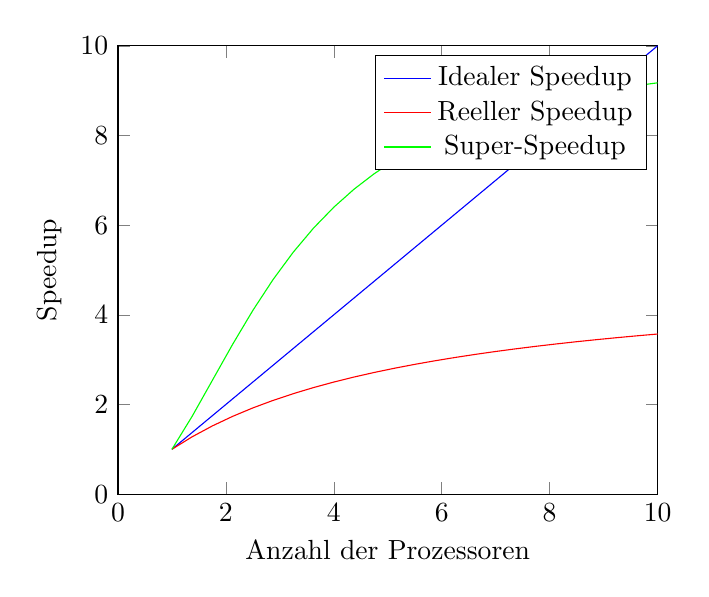
\begin{tikzpicture}
            \begin{axis}[
                xlabel={Anzahl der Prozessoren},
                ylabel={Speedup},
                xmin=0, xmax=10,
                ymin=0, ymax=10,
                legend entries={Idealer Speedup, Reeller Speedup, Super-Speedup}
              ]
              % Idealer Speedup
              \addplot[blue, domain=1:10] {x};

              % Reeller Speedup
              \addplot[red, domain=1:10] {x/(1 + (x-1) * 0.2)};

              % Superspeedup
              \addplot[green, domain=1:10] {x^3/(x + (x^3-x) * 0.1)};
            \end{axis}
          \end{tikzpicture}
          \caption{Speedup}
          \label{fig:speedup}
        \end{figure}

        In der Grafik~\ref{fig:speedup} repräsentiert die blaue Linie den idealen Speedup, bei dem die Leistung linear mit der Anzahl der Prozessoren zunimmt. Die rote Linie zeigt den realen Speedup, der in der Regel geringer als der ideale Speedup ist. Die letzte Kurve beschreibt den Super-Speedup.
        In verteilten Systemen kann ein sogenannter \enquote{Superspeedup} erreicht werden, wenn die Berechnungen und Prozesse über mehrere Rechner oder Knoten verteilt werden, was zu einer signifikanten Verbesserung der Leistung führt und zusätzlich Caching Mechanismen genutzt werden, die auf einer einzelnen CPU nicht möglich wären.\\
        \\
        Wie auch immer, zu Beginn der Entwicklung eines Verteilten Systems steht häufig noch nicht fest, inwieweit das System langfristig skalieren soll, daher sind auch schon kleine Systeme mit ausreichend Skalierungsmöglichkeiten zu designen und damit auch mit einem hohen Maß an möglicher Parallelität. Dies kann in kleinen Entscheidungen bereits einen großen Unterschied machen, wie beispielhaft in der Auswahl der Sortieralgorithmen.
\examplevs{ 
        \paragraph{Quicksort vs Mergesort in VS}\mbox{}\\
        Hier sollen beispielhaft zunächst zwei Gründe aufgeführt werden, warum die Auswahl von Mergesort sich in einer generischen Diskussion besser eignet, als die Wahl von Quicksort. Diese Diskussion soll einzig die Detailtiefe der Überlegungen andeuten.

        Zunächst steht hier der Kommunikationsaufwand: Bei Quicksort müssen die Teillisten für jeden rekursiven Aufruf aufgeteilt und zwischen verschiedenen Knoten im verteilten System ausgetauscht werden. Dies erzeugt einen hohen Kommunikationsaufwand zwischen den Knoten, der die Gesamtleistung des verteilten Systems beeinträchtigen kann. Im Gegensatz dazu kann Mergesort leichter parallelisiert werden, indem die sortierten Teillisten fusioniert werden, um die endgültige sortierte Liste zu erstellen. Hierdurch wird der Kommunikationsaufwand reduziert.

        Weiter existiert das Risiko des schlecht gewählten Pivot-Elements:
        Wenn das Pivot-Element nicht sorgfältig ausgewählt wird, kann dies zu einer ungleichmäßigen Verteilung der Arbeit führen. Ein schlecht gewähltes Pivot-Element kann dazu führen, dass eine Teilliste ungewöhnlich groß wird und mehr Zeit benötigt, um sortiert zu werden als die anderen Teillisten. Infolgedessen können einige Knoten im verteilten System stark belastet werden, während andere Knoten inaktiv bleiben, was die Gesamtleistung des Systems beeinträchtigt.

        Dies macht deutlich, dass bei der Konzeptionierung eines skalierenden Systems, nicht nur Anforderungen an das Problemverständnis gestellt werden, sondern auch eine breite Expertise. Diese umfasst eine tiefe Kenntnis über die möglichen Lösungskorridore  und ihrer bestimmenden Eigenschaften.
}
        Am Ende sollte noch eine weitere Gesetzmäßigkeit  für die Skalierung verinnerlicht werden. Brooks sagt aus, dass die Komplexität eines Systems nicht durch Hinzufügen von Ressourcen reduziert werden kann. 
\warningvs{Mit anderen Worten, wenn ein System zu komplex ist, wird es nicht einfacher, nur weil man mehr Ressourcen hinzufügt.}Diese Gesetzmäßigkeit wird aber viel zu oft in der Praxis ignoriert. Jeder Knoten muss mit den neuen Knoten interagieren, was den Kommunikationsaufwand exponentiell steigen lässt. Zudem entsteht zusätzlicher Overhead durch Synchronisation und Datenverteilung. Ein Beispiel ist ein verteiltes Datenbanksystem: Wenn zusätzliche Datenbankserver hinzugefügt werden, steigt der Aufwand für die Konsistenzsicherung und Partitionstoleranz.
  \item \textbf{Verwaltungs- oder Administrative-Skalierbarkeit}: Verwaltungs- oder administrative Skalierbarkeit bezieht sich auf die Fähigkeit eines verteilten Systems, effektiv und effizient von Administratoren oder Betreibern verwaltet und überwacht zu werden, unabhängig von der Größe oder Komplexität des Systems. Dies ist besonders wichtig, da verteilte Systeme in der Regel aus einer Vielzahl von Komponenten und Knoten bestehen, die auf verschiedenen Hardware- und Software-Plattformen laufen und in verschiedenen Netzwerken miteinander kommunizieren.

        Ein wichtiges Ziel der Verwaltungs- oder Administrative-Skalierbarkeit ist es, eine konsistente und zuverlässige Überwachung, Konfiguration und Verwaltung von verteilten Systemen zu ermöglichen, unabhängig von der Größe oder Komplexität des Systems. Dies kann durch die Verwendung von automatisierten Tools und Prozessen erreicht werden, die es Administratoren ermöglichen, das System zentralisiert und effektiv zu überwachen und zu verwalten.
\examplevs{
        Kubernetes ist ein in diesem Zusammenhang häufig genanntes Beispiel. Es handelt sich um eine Open-Source-Plattform für die Verwaltung von containerisierten Anwendungen. Kubernetes bietet eine Vielzahl von Funktionen und Werkzeugen, die es Administratoren ermöglichen, containerisierte Anwendungen unabhängig von der Größe oder Komplexität des Systems effizient zu verwalten. Dazu gehören Funktionen wie automatische Skalierung, Lastverteilung, Fehlerbehebung, Überwachung und Protokollierung.
}
\examplevs{
        Auch Apache ZooKeeper sollte genannt werden, als eine Open-Source-Software zur Koordination von verteilten Anwendungen. ZooKeeper bietet Funktionen wie Synchronisierung, Konfiguration, Überwachung und Benachrichtigung, die es Administratoren ermöglichen, komplexe verteilte Anwendungen effektiv und effizient zu verwalten und zu überwachen.
}
\end{itemize}

\subsubsection{Verteilungstransparenz}

Das Ziel der Verteilungstransparenz in verteilten Systemen bezieht sich darauf, dass Benutzer und Anwendungen nicht bewusst sein sollten, dass sie auf ein verteiltes System zugreifen, d.h. das verteilte System sollte für sie transparent sein. Dies bedeutet, dass der Benutzer oder die Anwendung keine Kenntnis von der Anzahl der Knoten im System, ihrer physischen Speicherorte, der Kommunikationsmechanismen oder der Art und Weise haben sollte, wie die Daten im System verteilt sind oder wie die Auslastung des Systems ist.
\\\\
Die Verteilungstransparenz ist in der Tat ein schwieriges Ziel, da es viele widersprüchliche Anforderungen gibt, die erfüllt werden müssen. Einerseits muss das verteilte System in der Lage sein, effektiv mit verschiedenen Komponenten und Knoten zu kommunizieren und Ressourcen zu teilen, andererseits darf dies jedoch nicht zu einer Beeinträchtigung der Leistung oder Verfügbarkeit des Systems führen. Darüber hinaus muss das verteilte System sicher und zuverlässig sein, um sicherzustellen, dass Daten und Informationen nicht kompromittiert werden oder verloren gehen.

Es ist daher richtig, dass die Verteilungstransparenz nie zu 100\% erreicht werden kann, da es immer einige Aspekte gibt, die für den Benutzer oder die Anwendung nicht transparent sind. Zum Beispiel kann die Latenzzeit bei der Übertragung von Daten zwischen verschiedenen Knoten im System nicht vollständig beseitigt werden, was zu einer gewissen Verzögerung führt.  Selbst Licht, so müssen wir feststellen, ist für die Kommunikation nicht selten zu langsam. Ebenso kann es aufgrund der Verteilung der Daten im System nicht immer möglich sein, einen vollständigen Überblick über alle Daten im System zu haben.
\\\\
Trotz dieser Herausforderungen ist die Verteilungstransparenz ein wichtiges Ziel in verteilten Systemen, da sie die Effizienz und Skalierbarkeit des Systems erhöht und die Komplexität und die Kosten reduziert. Obwohl die Verteilungstransparenz nie vollständig erreicht werden kann, gibt es verschiedene Technologien und Ansätze, die genutzt werden können, um sie zu verbessern, wie zum Beispiel Load Balancing, Replikation, Caching und Datenpartitionierung.

Da es ein schwieriges Feld ist dieses Ziel zu erreichen, greift der informierte Informatiker auch in diesem Fall nicht ungern wieder auf die Teile-und-herrsche Methode zurück, die es erlaubt die einzelnen Anforderungsaspekte besser zu verstehen und geeignet, des gewünschten Grades nach, umzusetzen:
\begin{itemize}
  \item  \textbf{Zugriffstransparenz (Access)}: Sie ist eine Art der Transparenz in verteilten Systemen, die darauf abzielt, dem Benutzer den Zugriff auf Ressourcen im Netzwerk so einfach wie möglich zu machen. Der Benutzer sollte in der Lage sein, auf Ressourcen zuzugreifen, ohne sich darüber Gedanken machen zu müssen, wo sich die Ressourcen befinden oder wie sie zugänglich gemacht werden können.

        Zugriffstransparenz kann gut am Beispiel der Dienstvermittlung diskutiert werden. Bei der Dienstvermittlung wird ein zentraler Dienst eingerichtet, der Benutzern dabei hilft, auf Ressourcen im Netzwerk zuzugreifen, ohne dass sie sich über den genauen Standort oder die Eigenschaften der Ressourcen Gedanken machen müssen. Der Dienst kann beispielsweise die Namen von Diensten und Ressourcen im Netzwerk bereitstellen und den Benutzer auf die entsprechenden Ressourcen weiterleiten.
\examplevs{
        Eine besondere Variante der Dienstvermittlung ist die Adressauflösung. Hierbei wird eine Adresse verwendet, um auf eine Ressource im Netzwerk zuzugreifen, ohne dass der Benutzer sich über den genauen Standort der Ressource Gedanken machen muss. Die Adressauflösung kann automatisch erfolgen, indem beispielsweise ein Domain Name System (DNS) verwendet wird.
}
        Auch Netzwerkprotokolle können im Sinne der Zugriffstransparenz diskutiert werden. Durch die Verwendung von Netzwerkprotokollen und damit verbundenen Schichtenmodellen können Benutzer auf Ressourcen im Netzwerk zugreifen, ohne sich Gedanken darüber machen zu müssen, wie die Kommunikation zwischen den Komponenten erfolgt oder wie Daten über das Netzwerk übertragen werden.

  \item \textbf{Lokalitäts-Transparenz (Location)}: Diese Transparenz zielt darauf ab, dem Benutzer die Komplexität des Systems zu verbergen, indem ihm das \enquote{Gefühl} vermittelt wird, dass Ressourcen lokal verfügbar sind, auch wenn sie sich in Wirklichkeit an einem entfernten Ort befinden.
        %Mit anderen Worten, Lokalitäts-Transparenz bedeutet, dass der Benutzer nicht wissen oder sich darum kümmern muss, wo sich eine bestimmte Ressource im Netzwerk befindet oder wie sie zugänglich gemacht wird.
\examplevs{
        Ein Beispiel für Lokalitäts-Transparenz ist die Verwendung von virtuellen Ressourcen. Durch die Erstellung von virtuellen Ressourcen, wie virtuellen Maschinen oder virtuellen Festplatten, können Ressourcen im Netzwerk bereitgestellt werden, ohne dass der Benutzer sich Gedanken darüber machen muss, wo sich die physischen Ressourcen befinden.
}
\examplevs{
        Ein weiteres Beispiel für Lokalitäts-Transparenz ist die Verwendung von Dateisystemen. Durch die Verwendung von verteilten Dateisystemen kann der Benutzer auf Dateien zugreifen, ohne sich Gedanken darüber machen zu müssen, wo sich die Dateien im Netzwerk befinden. Das verteilte Dateisystem sorgt dafür, dass der Benutzer auf die Dateien zugreifen kann, als ob sie sich lokal auf seinem Gerät befinden.
}
        Lokalitäts-Transparenz kann auch durch die Verwendung von Replikation erreicht werden. Durch die Replikation von Ressourcen auf verschiedene Knoten im Netzwerk kann der Benutzer auf die Ressourcen zugreifen, ohne sich Gedanken darüber machen zu müssen, wo sich die Ressourcen befinden oder welche Knoten verfügbar sind.

  \item \textbf{Migrationstransparenz (Migration)}: %Die Transparenz ermöglicht den Benutzern, von einem Ort oder Gerät zu einem anderen zu wechseln, ohne dabei ihre Sitzung oder den Zugriff auf ihre Ressourcen zu verlieren. 
        Migrationstransparenz ermöglicht es dem Benutzer, nahtlos zwischen verschiedenen Geräten oder Standorten zu wechseln, ohne dass er seine Arbeit unterbrechen oder sich neu anmelden muss. Die Anwendung bleibt in Ihrer Natur die gleiche, nur die Umgebung in der Sie ausgeführt wird, ändert sich.

        Auch für die Migrationstransparenz ist die Verwendung von Virtualisierungstechnologien wichtig. Benutzer können ihre Arbeitsumgebung in einer virtuellen Maschine speichern und auf verschiedenen Geräten ausführen, ohne ihre Sitzung oder den Zugriff auf ihre Ressourcen zu verlieren. Wenn der Benutzer beispielsweise von einem Laptop zu einem Desktop-Computer wechselt, kann er einfach die virtuelle Maschine auf dem Desktop öffnen und seine Arbeit fortsetzen, ohne dass er seine Sitzung unterbrechen oder sich erneut anmelden muss.

        Weiter ist die Verwendung von Cloud-basierten Diensten ein gutes Beispiel für Migrationstransparenz. Durch deren Verwendung können Benutzer auf ihre Ressourcen zugreifen, unabhängig von ihrem Standort oder dem Gerät, das sie verwenden. Wenn der Benutzer beispielsweise von einem mobilen Gerät auf einen Desktop-Computer wechselt, kann er einfach auf sie zugreifen und seine Arbeit fortsetzen, ohne seine Sitzung unterbrechen zu müssen.

        Die Migrationstransparenz wird oft durch Mechanismen wie Sitzungs- und Zustandssynchronisierung, Lastverteilung und automatische Skalierung erreicht. Sitzungs- und Zustandssynchronisierung ermöglicht es Benutzern, ihre Sitzungen und Zustände zwischen verschiedenen Geräten oder Standorten zu synchronisieren. Lastverteilung und automatische Skalierung sorgen dafür, dass die Ressourcen im System je nach Bedarf automatisch skaliert und verteilt werden, um eine unterbrechungsfreie Benutzererfahrung zu gewährleisten.

  \item \textbf{Replikationstransparenz (Replication)}:  Auf replizierte Ressourcen zuzugreifen, ohne sich über die Anzahl der Replikate, deren Standort oder die zugrunde liegenden Mechanismen Gedanken machen zu müssen ist ein tolles Ziel. Die  Replikationstransparenz ermöglicht es Benutzern, auf replizierte Ressourcen zuzugreifen, als ob es nur eine einzige Ressource im System gäbe, im besten Fall eine kohärente.
\examplevs{
        Ein Beispiel für Replikationstransparenz ist die Verwendung von replizierten Datenbanken. Durch die Replikation von Datenbanken auf verschiedenen Knoten im Netzwerk kann der Benutzer auf die Datenbank zugreifen, ohne sich Gedanken darüber machen zu müssen, wo sich die Datenbank befindet oder welche Knoten verfügbar sind. Der Benutzer kann einfach auf die replizierte Datenbank zugreifen, als ob es nur eine einzige Datenbank im System gäbe.
}
        %Ein weiteres Beispiel für Replikationstransparenz ist die Verwendung von verteilten Dateisystemen. Durch die Replikation von Dateien auf verschiedenen Knoten im Netzwerk kann der Benutzer auf die Dateien zugreifen, ohne sich Gedanken darüber machen zu müssen, wo sich die Dateien befinden oder welche Knoten verfügbar sind. Der Benutzer kann einfach auf die replizierten Dateien zugreifen, als ob es nur eine einzige Datei im System gäbe.

        Die Replikationstransparenz wird oft durch Mechanismen wie Replikation, Konsistenz-Protokolle und Fehlertoleranz erreicht. Die Replikation sorgt dafür, dass Daten oder Ressourcen auf mehreren Knoten im Netzwerk dupliziert werden, um eine höhere Verfügbarkeit und Zuverlässigkeit zu gewährleisten. Konsistenz-Protokolle sorgen dafür, dass alle Replikate synchronisiert werden und dass Änderungen an einem Replikat auch auf allen anderen Replikaten propagiert werden. Fehlertoleranzmechanismen sorgen dafür, dass das System auch dann noch funktioniert, wenn ein oder mehrere Knoten im Netzwerk ausfallen oder nicht verfügbar sind.

  \item \textbf{Fehlertransparenz (Error)}: Eine hohe Fehlertransparenz bedeutet, dass Fehler schnell erkannt und gemeldet werden können und dass alle Beteiligten wissen, was getan werden muss, um das Problem zu lösen.

        Es gibt verschiedene Methoden, um die Fehlertransparenz zu verbessern, wie beispielsweise:
        \begin{itemize}
          \item Fehlermeldungen sollten klar und deutlich sein und die Benutzer auf die Ursache des Fehlers und die Schritte, die sie unternehmen müssen, um das Problem zu lösen, hinweisen. Im besten Fall können automatische Strategien selbständig den Fehler beheben.

          \item Eine Protokollierung der Ereignisse, die zu einem Fehler geführt haben, kann helfen, die Ursache des Problems zu identifizieren und zukünftige Fehler zu vermeiden.

          \item Durch regelmäßige Tests und Validierung von Systemen und Prozessen können Fehler frühzeitig erkannt und behoben werden.

          \item Eine angemessene Schulung der Benutzer und Mitarbeiter in Bezug auf die Funktionsweise des Systems und mögliche Fehlerquellen kann dazu beitragen, dass Fehler vermieden oder schnell behoben werden können.
        \end{itemize}
        Die Referenzliteratur kennt zudem noch \textbf{Concurrency} (Nebenläufigkeitstransparenz) und \textbf{Relocation} (Umplatzierung). 

        Concurrency, oder Nebenläufigkeitstransparenz, bezieht sich auf die Fähigkeit eines Systems, mehrere Vorgänge gleichzeitig auszuführen, sodass Nutzer die Illusion erhalten, als ob ihre Programme allein auf dem System laufen. 

        Relocation in verteilten Systemen bezieht sich auf die Fähigkeit des Systems, Komponenten (wie Prozesse, Dienste oder ganze Anwendungen) während ihrer Ausführung zwischen verschiedenen physischen oder virtuellen Maschinen zu verschieben. Hier kann man sicher die Frage stellen ob sie der Replikation- oder Migrationstransparenz nicht inharärent sind, dieser Diskussion möchte der Author aber nicht vorgreifen.
        \paragraph{Diskussion Incident Management}\mbox{}\\
        Immer mehr setzt sich auch der Gedanke durch aus Fehlern zu lernen. Dies ist vielmehr eine organisatorische Diskussion als eine technische. Dieser Prozess wird häufig als \enquote{Incident Management} bezeichnet. In diesem Prozess kann nicht das Fehlerverhalten im auftretenden Fall korrigiert werden, aber die darauffolgenden Situationen. Einfach gesprochen ist es das Ziel einen Fehler nicht zweimal zu machen. Dies ist ein langfristiges Ziel in verteilten Systemen um die Fehlertransparenz zu erhöhen.
        \\\\
        \textbf{Incident Management} zielt auf die schnelle Identifizierung, Analyse, Reaktion und Behebung von unerwarteten Ereignissen oder Störungen, die die normalen Abläufe eines Systems, einer Organisation oder eines Netzwerks beeinträchtigen können. Incident Management ist ein wichtiger Bestandteil des IT-Service-Managements (ITSM) und zielt darauf ab, die negativen Auswirkungen solcher Vorfälle auf Geschäftsprozesse und die Servicequalität zu minimieren. Es umfasst im Allgemeinen die folgenden Schritte:
        \begin{itemize}
          \item Incident-Erkennung: Das erste und entscheidende Element des Incident-Managements ist die frühzeitige Erkennung von Vorfällen. Dies kann durch automatisierte Überwachungssysteme, Benachrichtigungen von Benutzern oder Mitarbeitern oder andere Methoden erreicht werden.
          \item Incident-Registrierung: Sobald ein Vorfall erkannt wurde, wird er in einem zentralen Incident-Management-System (IMS) oder einem Ticketing-System erfasst. Dies stellt sicher, dass alle relevanten Informationen über den Vorfall dokumentiert sind und eindeutig identifiziert werden können.
          \item Incident-Klassifizierung: Nach der Registrierung wird der Vorfall anhand verschiedener Kriterien wie Dringlichkeit, Priorität und Auswirkung auf das Geschäft klassifiziert. Dies hilft dabei, Ressourcen und Maßnahmen angemessen zuzuordnen und die Reaktion auf den Vorfall effektiv zu steuern.
          \item Incident-Zuweisung: Basierend auf der Klassifizierung wird der Vorfall dem entsprechenden Support-Team oder Techniker zugewiesen, der die notwendige Expertise hat, um den Vorfall zu untersuchen und zu beheben.
          \item Incident-Untersuchung und Diagnose: Das Support-Team oder der Techniker untersucht den Vorfall, um die Ursache der Störung zu ermitteln, und entwickelt einen geeigneten Lösungsansatz.
          \item Incident-Behebung: Nach der Diagnose wird der identifizierte Lösungsansatz umgesetzt, um den Vorfall zu beheben und den betroffenen Service oder das System wieder in einen funktionsfähigen Zustand zu bringen.
          \item Incident-Schließung: Sobald der Vorfall erfolgreich behoben wurde und der betroffene Service oder das System wieder normal funktioniert, wird der Vorfall im Incident-Management-System geschlossen.
          \item Nachbereitung und Lernen: Nach dem Abschluss eines Vorfalls ist es wichtig, aus dem Vorfall zu lernen und Maßnahmen zu ergreifen, um ähnliche Vorfälle in der Zukunft zu verhindern oder die Reaktionszeit bei zukünftigen Vorfällen zu reduzieren. Dies kann durch Ursachenanalysen, Überprüfung der Prozesse und Implementierung von Verbesserungen erreicht werden.
        \end{itemize}
        Fehler sind kaum zu vermeiden, es sollte aber alles dafür getan werden, den Kunden nicht zu stark in die Fehlerhandhabung zu involvieren. Zumindest ist dies das Ziel der Fehlertransparenz.
\warningvs{Fehler ist keine Ausnahmesituation, sondern die Regel und sollte auch so im SE-Prozess von VS betrachtet werden. Es exisitiert nicht die Frage \enquote{ob} ein Fehler auftritt, nur \enquote{wann}.}
  \item \textbf{Ortstransparenz}: Sie ist eine weitere Art der Transparenz in verteilten Systemen, die oft in Zusammenhang mit Zugriffstransparenz steht. Sie bezieht sich darauf, dass der Benutzer nicht wissen muss, wo sich eine bestimmte Ressource im Netzwerk befindet, sondern nur wie er auf diese Ressource zugreifen kann, im besten Fall so, als ob sie sich lokal auf seinem Gerät oder innerhalb des Systems befindet.

        Die Implementierung des verteilten Systems selbst ist dafür verantwortlich, den Zugriff auf die Ressourcen im Netzwerk zu ermöglichen und die Komplexität des Systems vor dem Benutzer zu verbergen.

        Ortstransparenz wird oft durch Mechanismen wie Dienstvermittlung oder Adressauflösung erreicht. Adressauflösung sorgt dafür, dass der Benutzer auf eine Ressource zugreifen kann, ohne sich Gedanken darüber machen zu müssen, wo sich die Ressource im Netzwerk befindet.

  \item \textbf{Skalierbarkeits-Transparenz}: Skalierbarkeits-Transparenz bezieht sich auf die Fähigkeit eines Systems, seine Kapazität und Leistung zu erhöhen, wenn die Anforderungen steigen. Eine hohe Skalierbarkeits-Transparenz bedeutet, dass die Skalierung für die Benutzer und Kunden transparent und unkompliziert ist.

        Es gibt verschiedene Methoden, um die Skalierbarkeits-Transparenz zu verbessern, wie beispielsweise:
        \begin{itemize}
          \item Automatisierung: Durch die Automatisierung von Prozessen wie der Lastverteilung und Skalierung können die Ressourcen des Systems effektiv und automatisch verwaltet werden, ohne dass menschliche Eingriffe erforderlich sind.
          \item Virtualisierung: Durch die Virtualisierung von Hardware und Ressourcen können zusätzliche Ressourcen bei Bedarf schnell bereitgestellt werden, um den Anforderungen gerecht zu werden.
          \item Cloud Computing: Cloud-Computing-Plattformen bieten eine skalierbare Infrastruktur, die es Benutzern ermöglicht, schnell und einfach auf zusätzliche Ressourcen zuzugreifen, wenn sie benötigt werden.
          \item Überwachung und Messung: Durch die Überwachung der Systemleistung und Messung von Metriken wie der CPU-Auslastung und dem Netzwerkverkehr können Engpässe identifiziert und zusätzliche Ressourcen bereitgestellt werden.
          \item Architektur: Eine skalierbare Architektur, die auf verteilten Systemen und Microservices basiert, kann die Skalierbarkeit eines Systems verbessern, da einzelne Komponenten unabhängig voneinander skaliert werden können.
        \end{itemize}

\end{itemize}
\subsubsection{Kohärentes System}
Auch wenn die Verteilungstransparenz kaum erreicht werden kann, soll in der folgenden Diskussion davon ausgegangen werden. Durch die Erreichung wird eine wertvolle Eigenschaft für das verteilte System möglich, die sich am Ende auch wieder in viele Definitionen reiht:

\importantvs{Das System verhält sich dann wie ein kohärentes System für den Benutzer, so, als ob alle Daten und Funktionen, die er/sie verwendet oder abfragt, an einem zentralen meist lokalen Ort angeboten werden, obwohl die Daten in Wirklichkeit in verschiedenen Knoten im verteilten System umgesetzt und gespeichert sein können.}
\mbox{}Benutzer sollten keine Kenntnis davon brauchen, dass das System verteilt agiert. Der Benutzer muss auch nicht nur als Endanwender gesehen werden, sondern kann auch auf Anwendungsentwickler erweitert werden, die auf einem verteilten System ihre Anwendungen umsetzen.
So kann auch eine andere Software diese Eigenschaft nutzen, als ob sie mit einem monolithischen System interagiert, was viele Dinge für den Anwendungsentwickler stark vereinfacht.
\examplevs{
\textbf{Analogie für kohärenten System}
\\\\
In einer Küche arbeitet ein Koch-Team oft gemeinsam an der Zubereitung von Mahlzeiten. Jeder Koch hat seine spezifischen Aufgaben, wie das Schneiden von Gemüse oder das Kochen von Fleisch. Obwohl jeder Koch unterschiedliche Aufgaben hat und möglicherweise auf verschiedene Geräte und Zutaten zugreift, arbeiten sie alle zusammen, um sicherzustellen, dass die Mahlzeit auf den Tisch kommt.

Ein kohärentes System in einem verteilten System kann ähnlich funktionieren. Jeder Knoten im System kann spezifische Daten oder Ressourcen haben, auf die nur er zugreifen kann. Aber wie in der Küche arbeiten alle Knoten im System zusammen, um sicherzustellen, dass die Anwendung oder das System als Ganzes einheitlich und kohärent ist.

Wenn ein Benutzer, wie ein Kellner, eine Anfrage an das System sendet, weiß er/sie nicht, welcher Knoten im System die Anfrage bearbeitet. Wenn ein kohärentes System gut funktioniert, dann sollte es für den Benutzer so transparent wie möglich sein, so wie ein Team von Köchen, das sich wie ein einzelner Koch verhält. Diese Idee wird im Architekturkapitel auch nochmal aufgenommen, wie auch andere hier bisher nur kurz eingeführte Begriffe.
}

\subsection{Ziele im Anforderungsprozess}
Die Ziele eines Verteilten Systems spielen eine wichtige Rolle im Anforderungsprozess für das Design und die Entwicklung. Wenn ein Verteiltes System entworfen und entwickelt wird, müssen die Ziele und Anforderungen des Systems klar definiert sein, um sicherzustellen, dass das System die beabsichtigten Ziele und die Anforderungen erfüllt. Dies ist leichter gesagt, als getan.

Ein Anforderungsprozess für Verteilte Systeme sollte in mehrere Schritte unterteilt werden, die sich insbesondere am Anfang auf die Definition, Erfassung und Verwaltung der Anforderungen konzentriert. Dies wird auch nochmals deutlicher in der mit diesem Script verbundenen praktischen Arbeit. \examplevs{
Im Folgenden werden einige der bisher genannten Schritte im Anforderungsprozess beschrieben\footnote{Eine Auseinandersetzung mit diesen Schritten, wird für die praktische Aufgabe sehr empfohlen}:
\begin{itemize}
  \item \textbf{Definieren der Ziele und Anforderungen:} Das erste und wichtigste Ziel im Anforderungsprozess ist die Ziele und Anforderungen des Verteilten Systems zu definieren. Dies auch im Detail mit Fokus auf Priorität und  Ausprägung.
\end{itemize}
}
\examplevs{
\begin{itemize}
  \item \textbf{Anforderungen erfassen:} Nachdem die Ziele und Anforderungen definiert wurden, müssen sie erfasst und dokumentiert werden. Hierbei können Techniken wie Interviews, Umfragen, Workshops oder Prototyping genutzt werden, um die Bedürfnisse und Anforderungen der Benutzer und Stakeholder des Systems zu ermitteln. Die Auseinandersetzung mit Software Engineering Werkzeugen wird sehr angeraten. Auch kommt der Dokumentationsmethodik eine besondere Bedeutung zu. Werkzeuge wie ARC42\footnote{\url{https://www.arc42.de/overview/}} sind gut geeignet den Prozess zu steuern und zu organisieren.
\end{itemize}
}
\examplevs{
\begin{itemize}
  \item \textbf{Anforderungen analysieren und spezifizieren:} Die erfassten Anforderungen müssen analysiert und spezifiziert werden, um sicherzustellen, dass sie vollständig, konsistent und widerspruchsfrei sind. Hierbei können Methoden wie Use-Case-, Datenfluss- oder Zustandsdiagramme eingesetzt werden. Eine ausreichende Kenntnis der Beschreibung ist hier dringend geboten\footnote{UML Tutorial: \url{ http://bedford-computing.co.uk/learning/wp-content/uploads/2016/09/UML-2.0-in-Action_-A-project-based-tutorial-eBook.pdf}}.
\end{itemize}
}
\examplevs{
\begin{itemize}
  \item \textbf{Validieren und verifizieren der Anforderungen:} Die spezifizierten Anforderungen müssen anschließend validiert und verifiziert werden, um sicherzustellen, dass sie den Zielen und Anforderungen entsprechen und vollständig sind. Hierbei können Techniken wie Prototyping, Simulationen oder Tests eingesetzt werden. Auch Gespräche in der Fachgruppe sind hilfreich. Dies sollte begleitend zum Script in praktischen Übungen umgesetzt werden.
\end{itemize}
}
\examplevs{
\begin{itemize}
  \item \textbf{Verwalten der Anforderungen:} Schließlich müssen die Anforderungen verwaltet werden, um sicherzustellen, dass sie während des gesamten Lebenszyklus des Verteilten Systems aktuell und gültig bleiben. Hierbei können Tools und Techniken wie Anforderungsmanagement-Systeme oder Versionskontrollsysteme eingesetzt werden. Ideen wie Kanban Board können hier ein ersten Einstieg bieten.
\end{itemize}
}
Die Anforderungsanalyse für Verteilte Systeme ist ein wichtiger Schritt, um die Funktionalität, Leistung und Zuverlässigkeit eines verteilten Systems zu definieren und zu gewährleisten. 
\examplevs{
Hier sind einige Ansätze und Methoden, um eine Anforderungsanalyse für verteilte Systeme durchzuführen:
\begin{itemize}
  \item \textbf{Anwendungsfalldiagramme (Use Case Diagrams):} Diese Diagramme beschreiben die Interaktionen zwischen den Benutzern und dem System in Form von Anwendungsfällen. Bei verteilten Systemen ist es wichtig, die Kommunikation zwischen den verschiedenen Komponenten und die Verantwortlichkeiten jedes Systems zu identifizieren.

        Beispiel: Ein Anwendungsfalldiagramm für ein verteiltes E-Commerce-System könnte Anwendungsfälle wie Artikel suchen, Artikel kaufen und Bestellstatus überprüfen enthalten, die die Interaktionen zwischen Benutzern und verschiedenen Systemkomponenten darstellen.

  \item \textbf{Datenflussdiagramme (Data Flow Diagrams):} Diese Diagramme zeigen, wie Daten zwischen den verschiedenen Komponenten eines verteilten Systems fließen. Sie helfen dabei, die Abhängigkeiten zwischen den Systemen zu identifizieren und auf Datenzugriffsprobleme hinzuweisen.

        Beispiel: Ein Datenflussdiagramm für ein verteiltes Content-Management-System könnte den Fluss von Daten zwischen Webservern, Datenbanken und externen Diensten wie Authentifizierungsdiensten darstellen.

  \item \textbf{Architekturdiagramme:} Diese Diagramme geben einen Überblick über die Systemkomponenten und ihre Beziehungen zueinander. Sie können verwendet werden, um das Gesamtbild der Systemstruktur und die Verteilung von Funktionen über verschiedene Komponenten zu verstehen.

        Beispiel: Ein Architekturdiagramm für ein verteiltes Cloud-Computing-System könnte die Beziehungen zwischen Front-End-Servern, Backend-Servern, Datenbanken und Storage-Einheiten darstellen.
\end{itemize}
}
\examplevs{
\begin{itemize}
  \item \textbf{Qualitätsattribute und Szenarien:} Bei der Analyse von Anforderungen für verteilte Systeme ist es wichtig, Qualitätsattribute wie Leistung, Skalierbarkeit, Verfügbarkeit, Sicherheit und Wartbarkeit zu berücksichtigen. Das Definieren von Szenarien hilft dabei, die Anforderungen in Bezug auf diese Qualitätsattribute zu verstehen und zu priorisieren.

        Beispiel: Bei einem verteilten Video-Streaming-System könnten Qualitätsattribute wie niedrige Latenz, hohe Verfügbarkeit und Skalierbarkeit im Vordergrund stehen. Szenarien könnten das Hinzufügen neuer Server bei steigender Last oder das Wiederherstellen des Systems nach einem Ausfall umfassen.

  \item \textbf{Interview- und Workshop-Methoden:} Die Befragung von Stakeholdern und die Durchführung von Workshops ist ein wichtiger Ansatz, um Anforderungen für verteilte Systeme zu erheben und zu validieren. Befragungstechniken können strukturiert, halbstrukturiert oder unstrukturiert sein.

        Beispiel: Ein Workshop zur Identifizierung von Anforderungen für ein verteiltes Fertigungssystem könnte Stakeholder wie Produktmanager, Entwickler, Betriebsteams und Endbenutzer zusammenbringen, um gemeinsam Anforderungen zu definieren.
\end{itemize}
}
In dieser Ausarbeitung wird die perfekte Umsetzung der Diagramme nicht in den Fokus gestellt, sondern vielmehr Ihren Nutzen bei der Strukturierung und Visualisierung.

\subsection{Pitfalls}

Neben den Dingen, die man sich bewusst sein sollte, um sie gut zu machen, sollte man auch Dinge angehen, die dazu beitragen, immer wiederkehrende Fehler zu vermeiden.

\importantvs{Diese falschen Annahmen in verteilten Systemen, welche als \enquote{The Eight Fallacies of Distributed Computing} bekannt sind, haben eine hohe Bedeutung, sodass nicht wenige es als \enquote{Gesetz} beschreiben. Dieses \enquote{Gesetz} wurde von L. Peter Deutsch, einem Informatiker und Pionier im Bereich der verteilten Systeme, formuliert und beschreibt die falschen Annahmen, die oft in verteilten Systemen gemacht werden.
}
\begin{itemize}
  \item \textbf{Das Netzwerk ist immer verfügbar}: Diese Annahme geht davon aus, dass das Netzwerk immer verfügbar und zuverlässig ist und dass das System immer in der Lage ist, auf das Netzwerk zuzugreifen.

        In der Realität kann es jedoch jederzeit zu Netzwerkstörungen oder Ausfällen kommen, die das System beeinträchtigen können. Diese Störungen können durch physische Schäden, Überlastung oder andere Faktoren verursacht werden.

        Es ist wichtig, dass Entwickler bei der Gestaltung von verteilten Systemen diese Annahme nicht treffen und das System so gestalten, dass es auf Netzwerkstörungen vorbereitet ist. Dies kann durch die Implementierung von Redundanz und Failover-Mechanismen erreicht werden, die sicherstellen, dass das System auch bei einem Netzwerkausfall weiterhin funktioniert.

        Redundanz kann durch das Hinzufügen von zusätzlichen Knoten oder Kopien von Daten erreicht werden, die das System in der Lage machen, den Ausfall eines Knotens oder einer Datenbank zu überstehen. Failover-Mechanismen können automatisch ausgelöst werden, wenn ein Knoten oder eine Datenbank ausfällt, um den Betrieb des Systems auf einem anderen Knoten oder einer anderen Datenbank fortzusetzen.

  \item \textbf{Die Latenzzeit ist 0}: Diese Annahme geht davon aus, dass die Übertragung von Daten zwischen verschiedenen Knoten im System sofort und ohne Verzögerung erfolgt.

        In der Realität kann die Latenzzeit jedoch aufgrund von verschiedenen Faktoren wie der Entfernung zwischen den Knoten, der Netzwerklast und der Art der Übertragung nicht null sein. Eine Latenzzeit kann die Leistung von verteilten Systemen beeinträchtigen und dazu führen, dass Benutzer eine Verzögerung oder Wartezeit bei der Interaktion mit dem System erfahren.
        Caching kann verwendet werden, um häufig verwendete Daten im lokalen Speicher eines Knotens zu speichern, um die Latenzzeit bei wiederholten Anforderungen zu reduzieren. Pufferung kann verwendet werden, um die Verzögerung bei der Übertragung von Daten zwischen Knoten zu minimieren, indem Daten zwischengespeichert werden, bis sie vollständig übertragen sind.
  \item \textbf{Die Bandbreite ist unbegrenzt}: Diese Annahme geht davon aus, dass das Netzwerk immer genügend Bandbreite hat, um alle Anforderungen des Systems zu erfüllen.

        In der Realität kann die Bandbreite jedoch begrenzt sein, insbesondere in Situationen, in denen viele Benutzer oder Knoten im System gleichzeitig auf das Netzwerk zugreifen. Begrenzte Bandbreiten können die Leistung von verteilten Systemen beeinträchtigen und dazu führen, dass Benutzer längere Wartezeiten und Verzögerungen bei der Verwendung des Systems erfahren.
        Datenkomprimierung kann verwendet werden, um die Größe von Daten zu reduzieren, die zwischen Knoten im System übertragen werden, um die Nutzung der verfügbaren Bandbreite zu optimieren. Caching und Pufferung können verwendet werden, um Daten zwischenzuspeichern und die Bandbreitennutzung zu optimieren, indem Übertragungen reduziert werden und Wartezeiten bei der Übertragung minimiert werden.
  \item \textbf{Das Netzwerk ist sicher}: Diese Annahme geht davon aus, dass Daten im Netzwerk sicher sind und nicht von Dritten abgefangen oder manipuliert werden können.

        In der Realität kann das Netzwerk jedoch anfällig für verschiedene Arten von Angriffen sein, einschließlich Hacking, Phishing, Malware-Infektionen und anderen Bedrohungen. Diese Bedrohungen können dazu führen, dass Daten im Netzwerk gestohlen, beschädigt oder manipuliert werden, was zu Datenschutzverletzungen, Betriebsstörungen oder anderen Problemen im System führen kann.

        Verschlüsselung kann verwendet werden, um Daten im Netzwerk zu schützen, indem sie verschlüsselt werden, um sie für Dritte unlesbar zu machen. Authentifizierung und Zugriffskontrolle können verwendet werden, um sicherzustellen, dass nur autorisierte Benutzer auf das System zugreifen können und dass alle Aktivitäten im System überwacht werden, um potenzielle Sicherheitsbedrohungen zu erkennen und darauf zu reagieren.

  \item \textbf{Topologie ändert sich nicht}:
        Diese Annahme geht davon aus, dass die Struktur des Netzwerks stabil bleibt und dass sich keine Veränderungen ergeben, die die Kommunikation zwischen verschiedenen Knoten beeinträchtigen können.

        In der Realität kann die Topologie des Netzwerks jedoch unvorhersehbaren Veränderungen unterworfen sein, die die Kommunikation zwischen Knoten im System beeinträchtigen können. Diese Veränderungen können durch Faktoren wie Netzwerkverstopfung, Ausfälle von Knoten, Änderungen der Netzwerkkonfiguration und andere Faktoren verursacht werden.
        Zum Beispiel können dynamische Routing-Algorithmen und adaptive Netzwerkprotokolle verwendet werden, um Veränderungen in der Netzwerkumgebung zu erkennen und automatisch auf diese Veränderungen zu reagieren, indem sie die Routing-Tabellen aktualisieren und die Kommunikation zwischen Knoten im System optimieren.

  \item \textbf{Es gibt nur einen Administrator}: Diese Annahme geht davon aus, dass es nur einen Administrator im System gibt, der für alle Aspekte des Systems verantwortlich ist.

        In der Realität kann es jedoch mehrere Administratoren geben, die für verschiedene Teile des Systems oder für verschiedene Standorte oder Abteilungen zuständig sind. Jeder Administrator hat möglicherweise unterschiedliche Kenntnisse, Fähigkeiten und Zugriffsrechte, die sich auf die Leistung und Sicherheit des Systems auswirken können.
        Zum Beispiel können rollenbasierte Zugriffsrechte und Verwaltungstools verwendet werden, um sicherzustellen, dass Administratoren nur auf die Bereiche des Systems zugreifen können, für die sie zuständig sind, und dass alle Aktivitäten im System überwacht werden, um potenzielle Probleme oder Bedrohungen frühzeitig zu erkennen und darauf zu reagieren.

  \item \textbf{Transportkosten sind null}:
        Diese Annahme geht davon aus, dass es keine Kosten oder Einschränkungen gibt, wenn Daten zwischen verschiedenen Knoten im System transportiert werden.

        Zum Beispiel können Algorithmen zur Optimierung der Datenkomprimierung und Datenreduzierung verwendet werden, um die Menge an übertragenen Daten zu minimieren und die Kosten für den Datenverkehr zu reduzieren. Ebenso können Technologien wie Caching, Pufferung und Verteilung von Daten auf mehrere Knoten im System verwendet werden, um den Transport von Daten im System zu optimieren und die Kosten zu minimieren. Die Strategien sind sehr ähnlich zu der Annahme der unbegrenzten Bandbreite.
  \item \textbf{Das Netzwerk ist homogen}: Diese Annahme geht davon aus, dass alle Knoten im Netzwerk dieselbe Hardware- und Softwareumgebung haben und dass alle Knoten im System auf dieselbe Weise kommunizieren können.

        In der Realität können jedoch Knoten im Netzwerk unterschiedliche Hardware- und Softwareumgebungen haben, die sich auf die Leistung und Zuverlässigkeit des Systems auswirken können. Diese Unterschiede können zu Inkompatibilitäten und Problemen bei der Kommunikation zwischen Knoten im System führen.

        Zum Beispiel können Technologien und Protokollkonvertierung verwendet werden, um die Kommunikation zwischen Knoten im System zu erleichtern und sicherzustellen, dass Daten und Anwendungen in verschiedenen Umgebungen interoperabel sind.
\end{itemize}
Die \textbf{Fallacies of Distributed Computing} sollen Entwickler daran erinnern, dass verteilte Systeme komplexe Systeme sind und dass bestimmte Annahmen, die für zentrale Systeme gelten, in verteilten Systemen nicht unbedingt zutreffen. Durch das Verständnis dieser Fallacies können Entwickler bessere Entscheidungen treffen und bessere Systeme entwerfen, die die Herausforderungen der Verteilung bewältigen können. Dies alles muss in dem Anforderungsprozess seinen Raum finden.

\label{Woche02}

\end{document}